\documentclass[10pt,a4paper,oneside,twocolumn]{article}

    \usepackage{float}	% for floating figures (putting them anywhere we want
    \usepackage{amsmath}	% for maths
    \usepackage{graphicx}	% jpg
    \usepackage{hyperref}
    \usepackage{textcomp}
    \usepackage{verbatim}	% use of \begin{comment}
    \usepackage{pgfplots}	% use of pgf plots
    \usepackage{multicol}
    \usepackage[top=2cm, bottom=2cm, left=1.5cm, right=1.5cm]{geometry} %margins
    \usepackage{sidecap}	% for side captions
    \restylefloat{table}	% floating figures(Tables)
    \usepackage{caption}
    \captionsetup{justification=centering}
    \usepackage{subcaption}
    \usepackage{array}
    \usepackage{titlesec}
    \titleformat{\section}[block]{\Large\bfseries\filcenter}{}{1em}{}

    \newcommand{\red}[1]{\textcolor{red}{#1}} 
    \newcommand{\cyan}[1]{\textcolor{cyan}{#1}} 
    \newcommand{\blue}[1]{\textcolor{blue}{#1}} 
    \newcommand{\orange}[1]{\textcolor{orange}{#1}} 
    \newcommand{\purple}[1]{\textcolor{purple}{#1}} 
    \newcommand{\green}[1]{\textcolor{green}{#1}} 
    \definecolor{forestgreen}{RGB}{0,102,0}
    \newcommand{\fgreen}[1]{\textcolor{forestgreen}{#1}} 

    \numberwithin{equation}{section} %permits numbering within sections instead of globally
\begin{document}

\title{\huge{\textbf{Mini-Project in Mathematical and Computational Modeling}}\\
	\vspace{0.5cm}
	\Large{\textit{\'Ecole Polytechnique F\'ed\'erale de Lausanne, Switzerland}}}
\author{\large{Florian + Dariush}}
\twocolumn[{
    \centering
    \huge{\textbf{Mini-Project in Mathematical and Computational Modeling}} \\
    \vspace{0.5cm}
    \Large{\textit{\'Ecole Polytechnique F\'ed\'erale de Lausanne, Switzerland}}\\
    \vspace{0.5cm}
    \large{Florian + Dariush}
    \vspace{1cm}
	}]

    oalruechoaluerchoaeulrch

    \par
    \hfill \\
    In the following url you can find the collection of .gif files that we made to show the evolution of X in all N cells over time. \\
    \url{https://github.com/Afanc/mini-pro-model/tree/Florian/Miniprojet\%202.0/Part\%20C} \\
    In C\_2\_gif\_1 until C\_2\_gif\_6 we see the evolution of the complexity of our system. The titles in the .gif files give the indication as to what part of the model was added. A is the reference to the correlation matrix between the cells. Lambda refers to the multiplier of the period. N is the number of cells



    \begin{figure*}[!htb] 		%oh my god this is so ugly pls don't look at me
	\captionsetup{labelformat=empty}
	\caption{\Huge{\textbf{Part A - One-Cell Model}}}
    \end{figure*}
    \begin{figure*}[!htb]
	\begin{subfigure}[b]{0.5\textwidth}
	    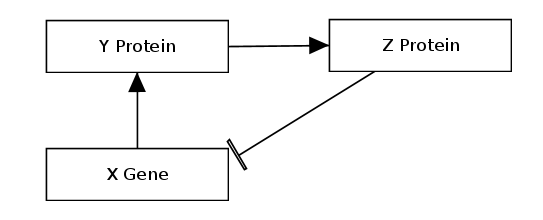
\includegraphics[width=\textwidth]{sketch.png}
	    \caption{
		One-Cell Model\\
	    The gene mRNA $X$ codes for protein $Y$ which, in turn, activates transcriptional inhibitor $Z$. The resulting model behaves as a three-variable oscillator.
	    }
	\end{subfigure}
	~
	\begin{subfigure}[b]{0.5\textwidth}
	    \begin{equation*}\frac{\delta X}{\delta t} = v_1 \frac{K_1^n}{K_1^n + Z^n} - v_2 \frac{X}{K_2 + X} \end{equation*}
	    \begin{equation*}\frac{\delta Y}{\delta t} = k_3 X - v_4 \frac{Y}{K_4 + Y}\end{equation*}
	    \begin{equation*}\frac{\delta Z}{\delta t} = k_5 Y - v_6 \frac{Z}{K_6 + Z}\end{equation*}

	    \captionsetup{labelformat=empty}
	    \caption{\\
	    \begin{tabular}{@{}>{$}l<{$}l @{\hskip 0.2cm} | @{\hskip 0.2cm} @{}>{$}l<{$}l@{}}
		v_1 & translation rate of $X$ & K_1 & Michaelis constant of $X$ \\
		v_2 & degradation rate of $X$ & K_4 & Michaelis constant of $Y$ \\
		v_4 & degradation rate of $Y$ & K_6 & Michaelis constant of $Z$\\
		v_6 & degradation rate of $Z$ &&\\
		k_3 & transcription rate of $Y$ && \\
		k_5 & transcription rate of $Z$ &&\\
	    \end{tabular}
	    }
	\end{subfigure}
    \end{figure*}

    \begin{figure*}[!h]
	\begin{subfigure}[b]{0.5\textwidth}
	    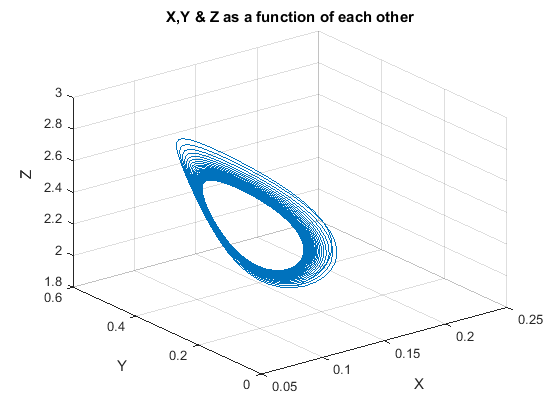
\includegraphics[width=\textwidth]{"../Miniprojet 2.0/Part A/A11.png}
	    \caption{Trajectories\\
	    The limit cycle is reached as the variations of $X(t)$, $Y(t)$ and $Z(t)$ become fixed : The trajectories converge, non-linearly (the distance between similar trajectories aren't regular) towards an elliptic limit cycle. The limit cycle is reached quickly due to favorable choice of initial conditions close to final concentrations. }
	\end{subfigure}
	~
	\begin{subfigure}[b]{0.5\textwidth}
	    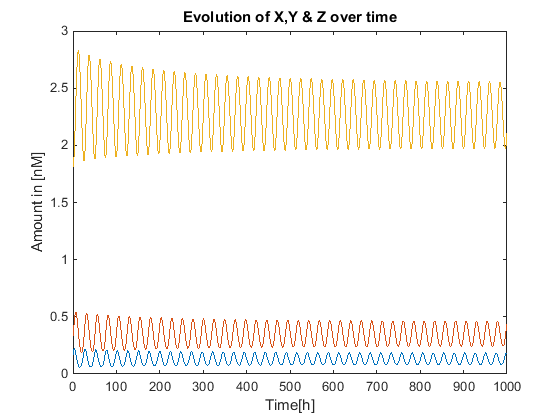
\includegraphics[width=\textwidth]{"../Miniprojet 2.0/Part A/A12.png}
	    \caption{Frequency spectrum \\
	    The amplitude of the three variations stabilize after a few hundred hours. The signal are not in phase but have the same, regular, frequencies.}
	\end{subfigure}
	\caption{\\Trajectories of $X(t)$, $Y(t)$ and $Z(t)$ with initial conditions : $X_0 = 0.16$, $Y_0 = 0.33 $, $Z_0 = 1.8$ [nM]\\ We observe on both graphs that $Z(t)$ has the bigger amplitude of variation whereas $X(t)$ and $Y(t)$ have small amplitudes. Additionally, the convergence towards a single loop in (a) indicate that the frequencies of the signals are equal; this is illustrated as well in (b)
	}
    \end{figure*}

    \begin{figure*}
    \centering
	\begin{subfigure}[b]{0.3\textwidth}
	    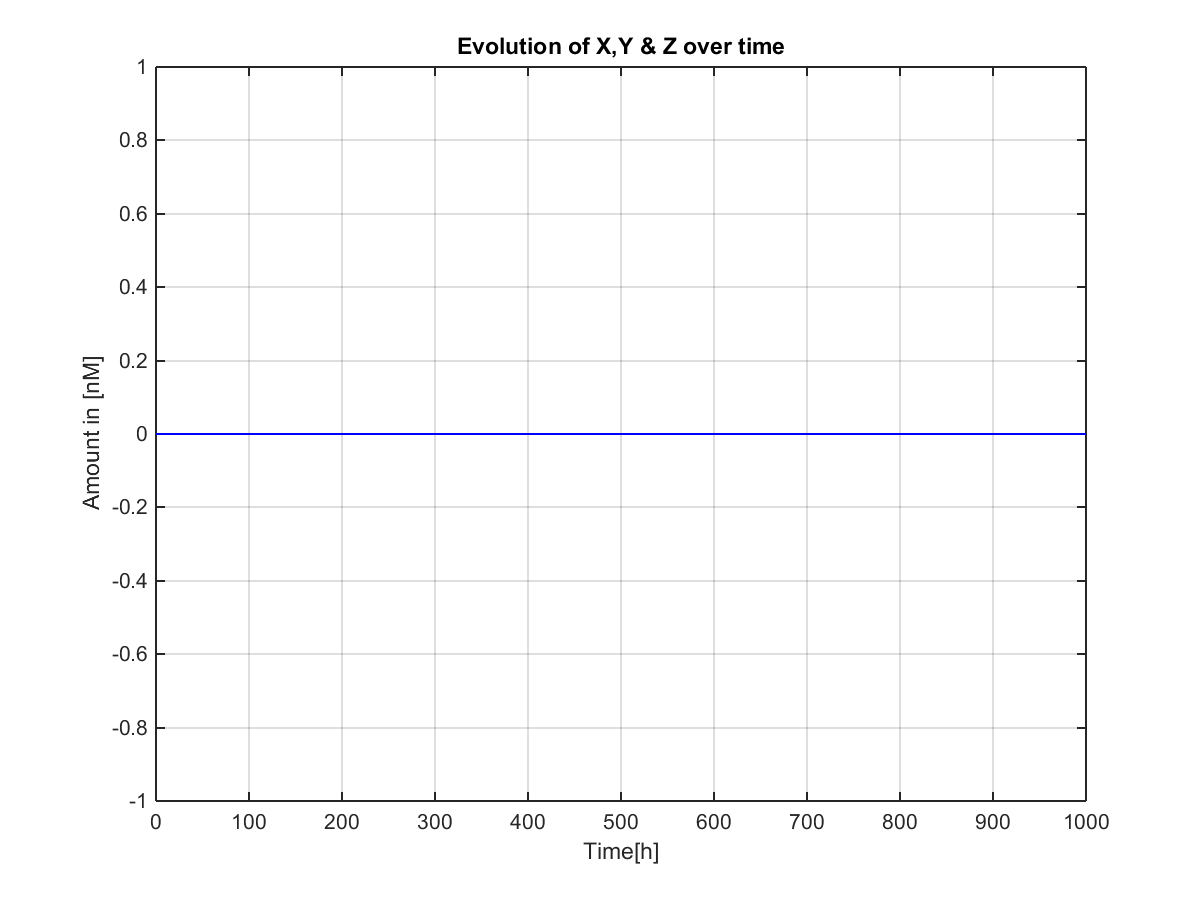
\includegraphics[width=\textwidth]{"../Miniprojet 2.0/Part A/A_3_graphs/A-A0.png}
	    \caption{$v_1$ = 0 nM/h}
	    \end{subfigure}
	    ~ 
	    \begin{subfigure}[b]{0.3\textwidth}
	    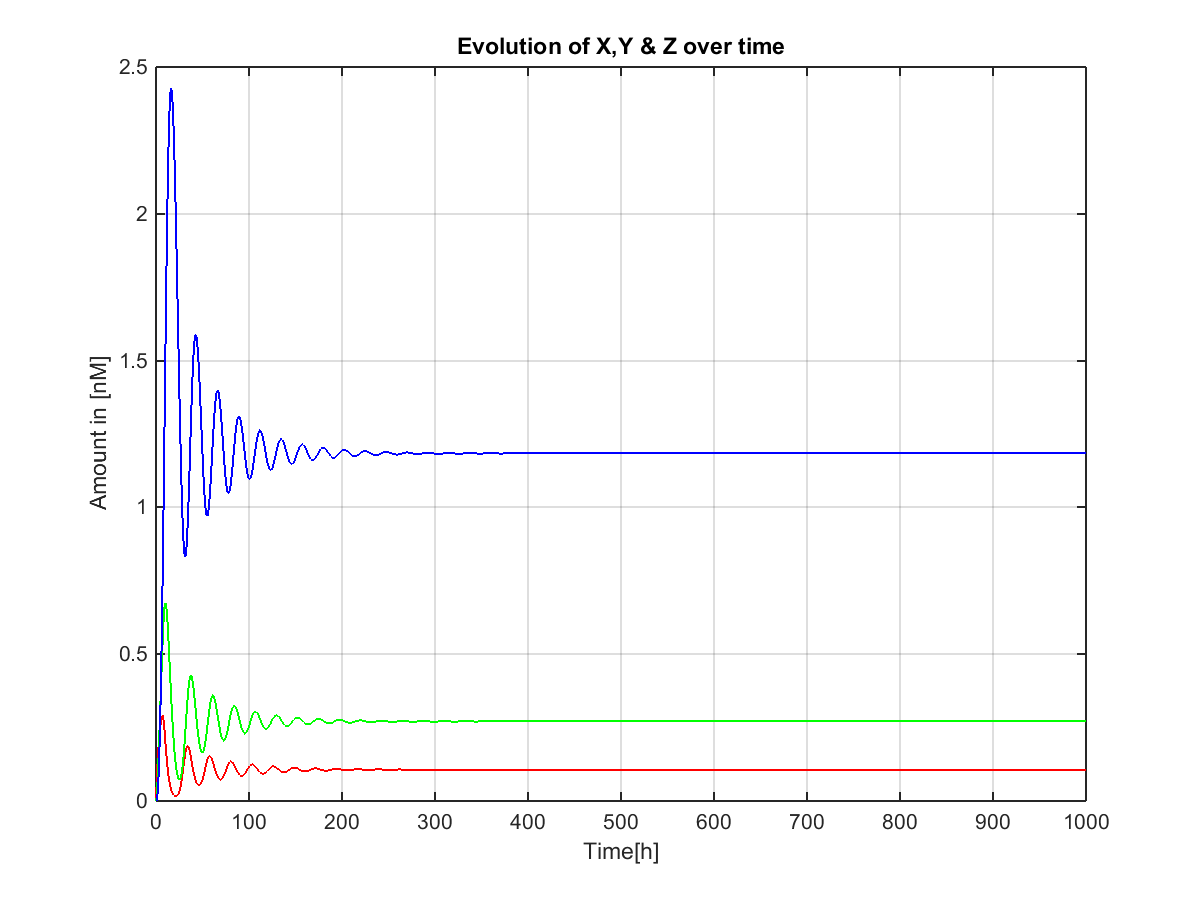
\includegraphics[width=\textwidth]{"../Miniprojet 2.0/Part A/A_3_graphs/A-A1.png}
	    \caption{$v_1$ = 0.1 nM/h}
	    \end{subfigure}
	    ~ 
	\begin{subfigure}[b]{0.3\textwidth}
	    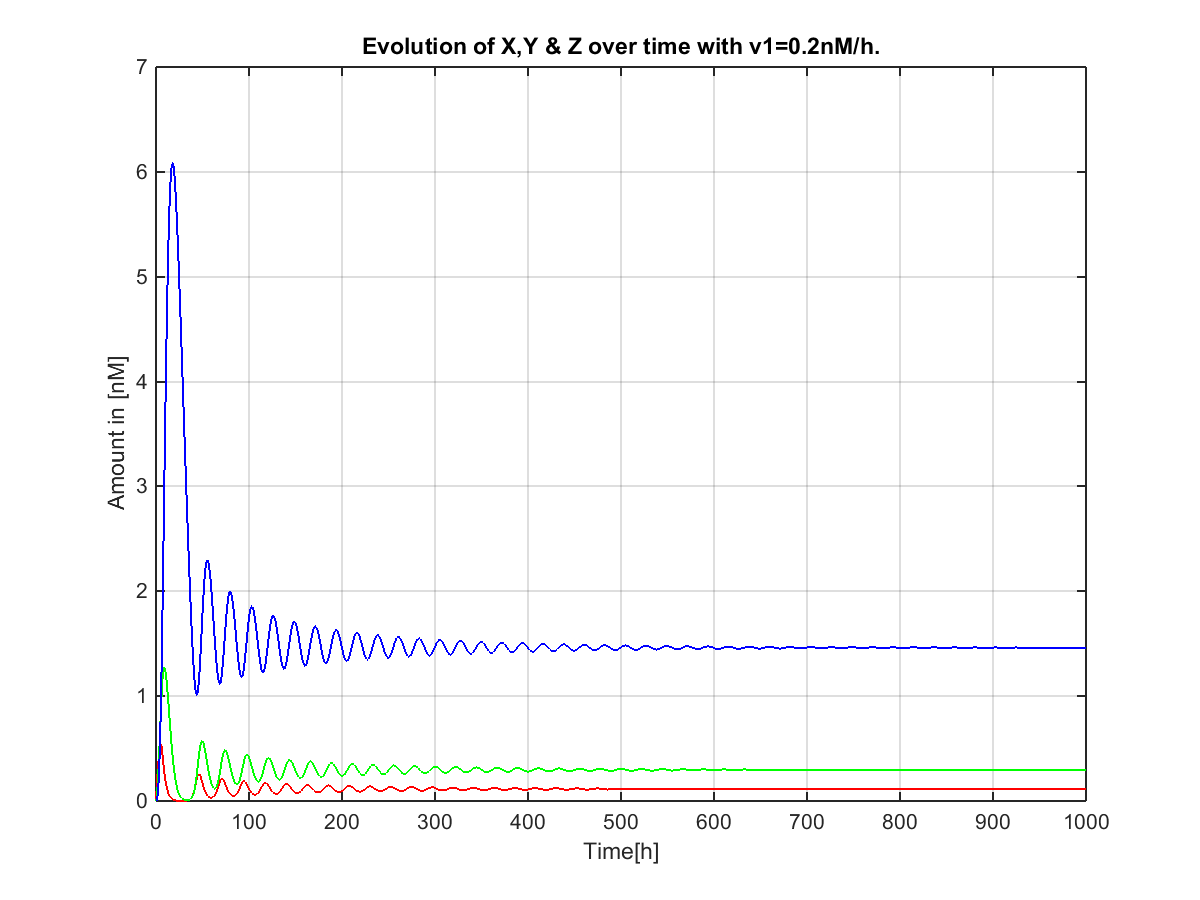
\includegraphics[width=\textwidth]{"../Miniprojet 2.0/Part A/A_3_graphs/A-A2.png}
	    \caption{$v_1$ = 0.2 nM/h}
	\end{subfigure}
	 
	\begin{subfigure}[b]{0.3\textwidth}
	    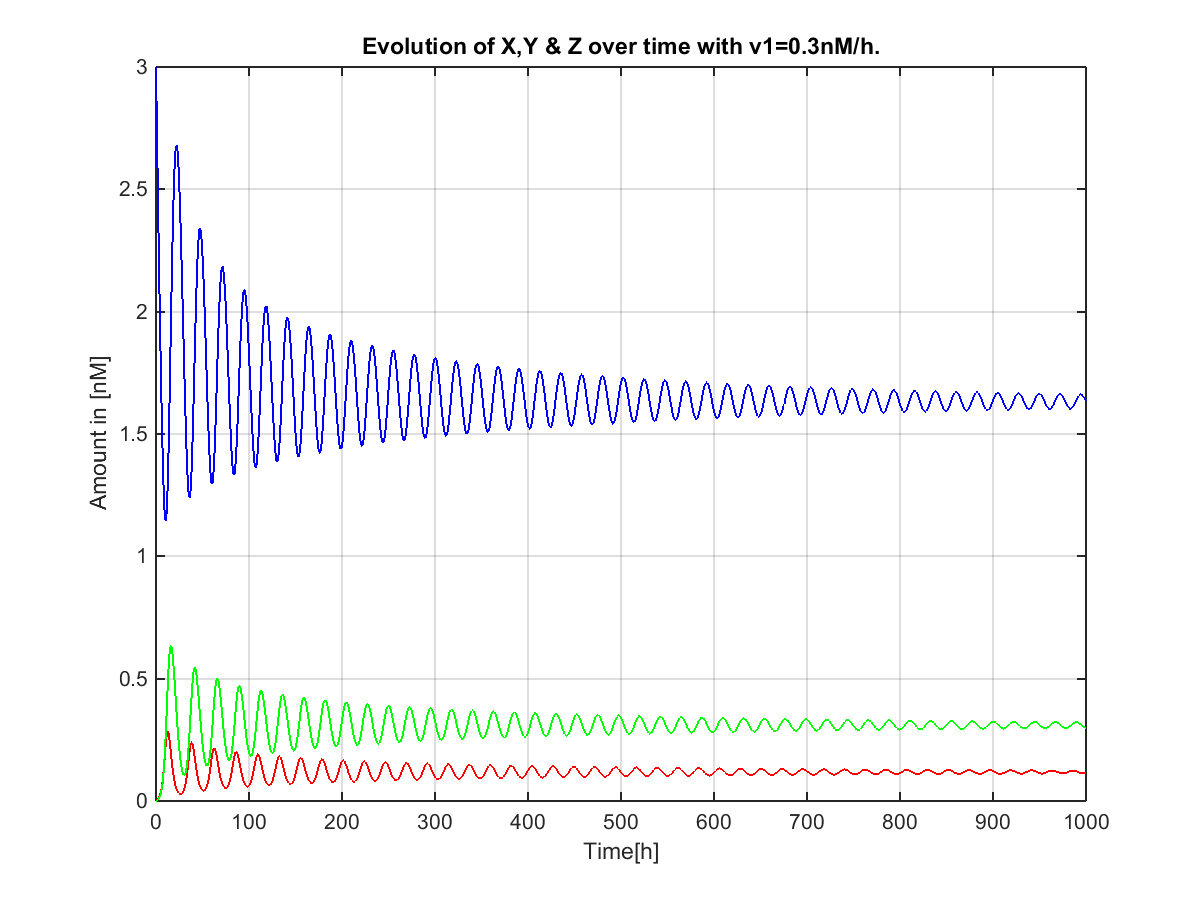
\includegraphics[width=\textwidth]{"../Miniprojet 2.0/Part A/A_3_graphs/A-A3.png}
	    \caption{$v_1$ = 0.3 nM/h}
	\end{subfigure}
	~ 
	\begin{subfigure}[b]{0.3\textwidth}
	    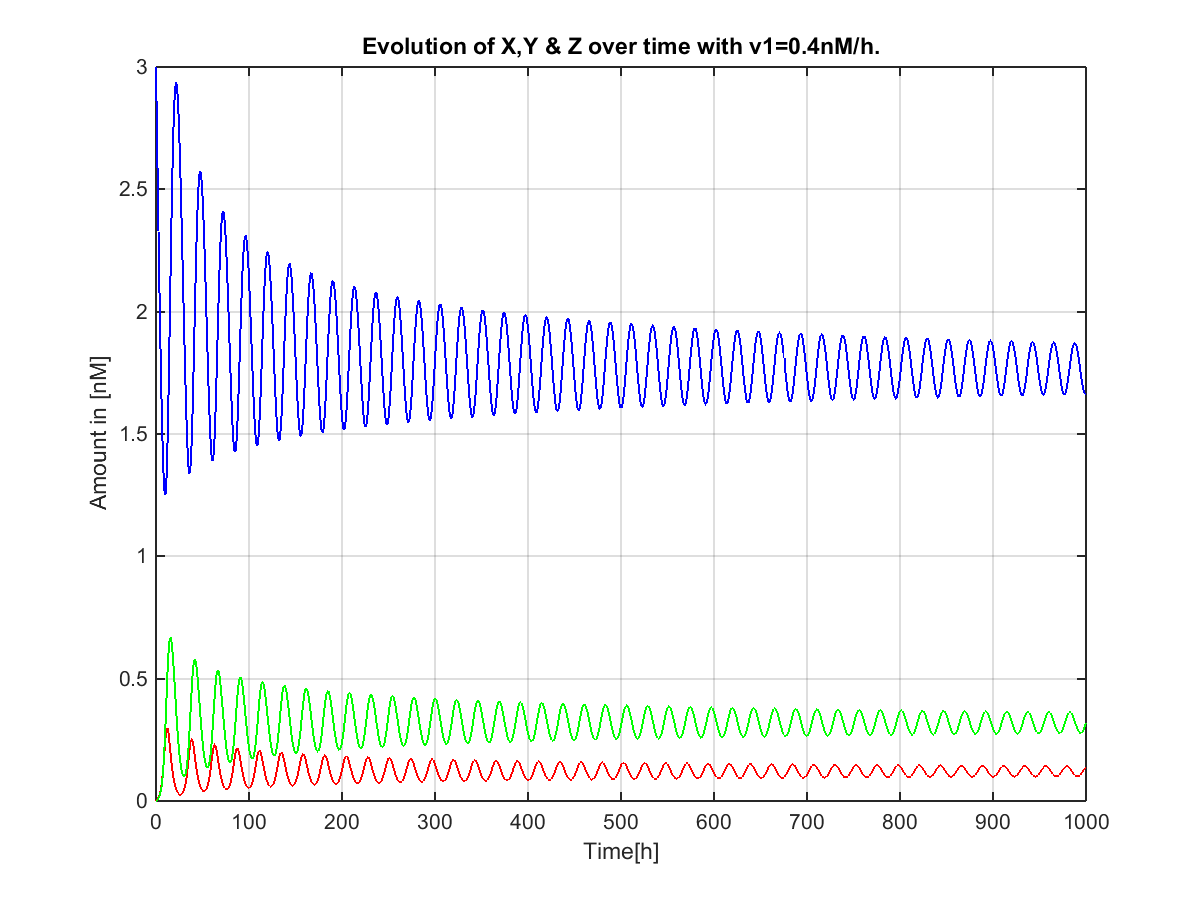
\includegraphics[width=\textwidth]{"../Miniprojet 2.0/Part A/A_3_graphs/A-A4.png}
	    \caption{$v_1$ = 0.4 nM/h}
	\end{subfigure}
	~
	\begin{subfigure}[b]{0.3\textwidth}
	    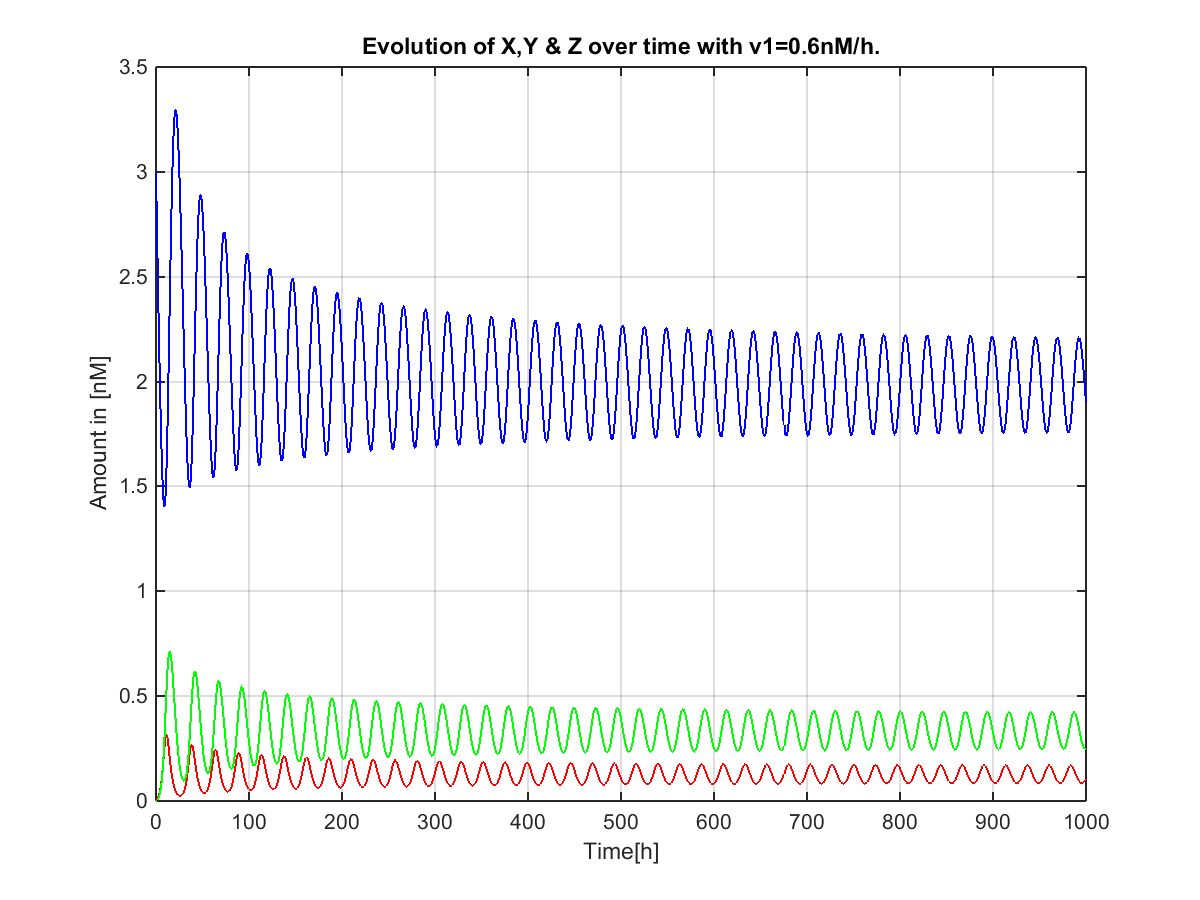
\includegraphics[width=\textwidth]{"../Miniprojet 2.0/Part A/A_3_graphs/A-A6.png}
	    \caption{$v_1$ = 0.6 nM/h}
	\end{subfigure}
	~ 
	\begin{subfigure}[b]{0.3\textwidth}
	    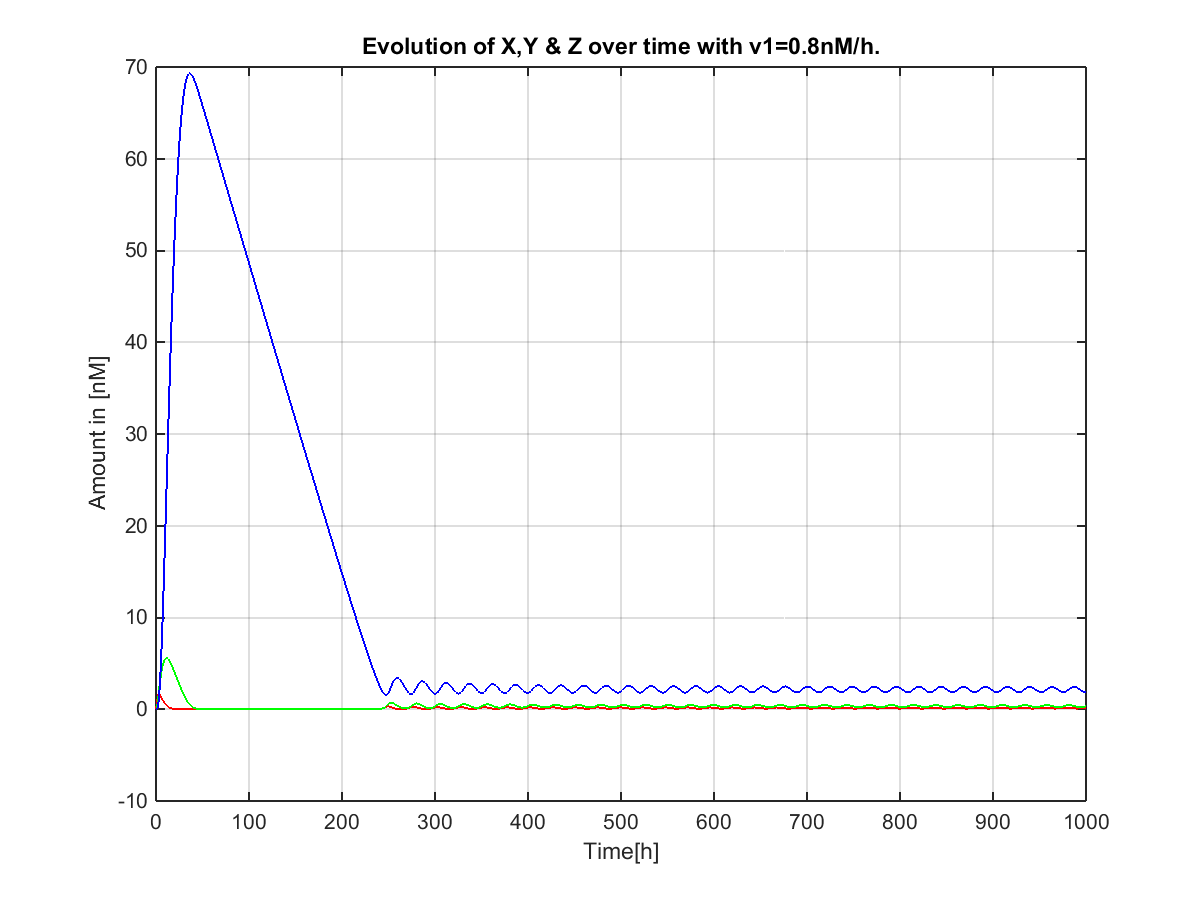
\includegraphics[width=\textwidth]{"../Miniprojet 2.0/Part A/A_3_graphs/A-A8.png}
	    \caption{$v_1$ = 0.8 nM/h}
	\end{subfigure}
	~
	\begin{subfigure}[b]{0.3\textwidth}
	    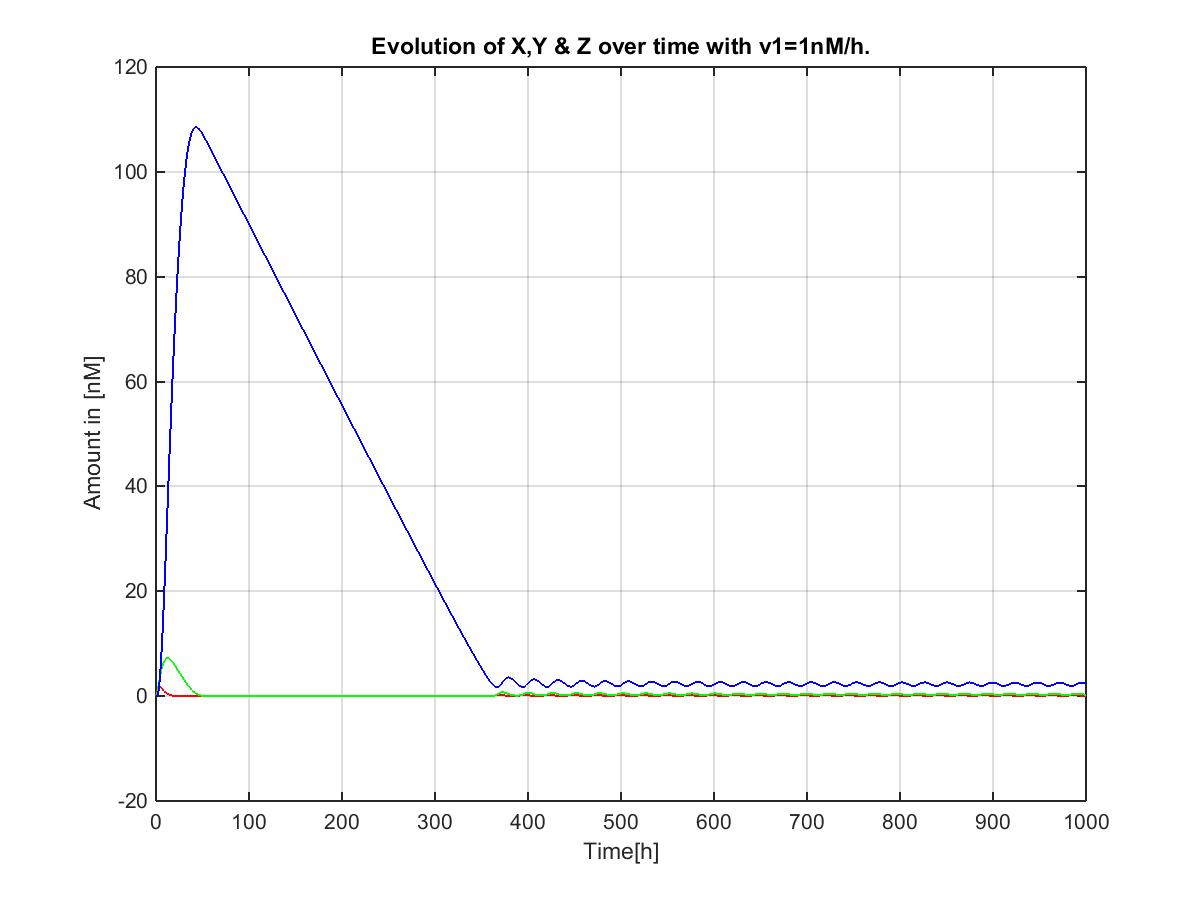
\includegraphics[width=\textwidth]{"../Miniprojet 2.0/Part A/A_3_graphs/A-A10.png}
	    \caption{$v_1$ = 1 nM/h}
	\end{subfigure}

	\caption{\green{$X(t)$}, \red{$Y(t)$} and \blue{$Z(t)$} with initial conditions $X_0 = 0.16$, $Y_0 = 0.33 $, $Z_0 = 1.8$ [nM]\\
	The first signal to fade is $Y(t)$ and its oscillatory stability predicts stability of the system. We also observe that the signals converge towards null, a fixed point or the limit cycle in a non-linear fashion. It is hard to precisely know the value for $v_1$ for which the system begins to display circadian behaviour, but it must be somewhere around $v_1$ = 0.5nM/h. A more accurate estimate will be made in the bifurcation diagram that follows. Interesting here is that the concentrations will reach a stable fixed point if $v_1$ is below a certain threshold. }
    \end{figure*}

    \begin{figure*}
	\centering
	    \begin{subfigure}[b]{0.35\textwidth}
		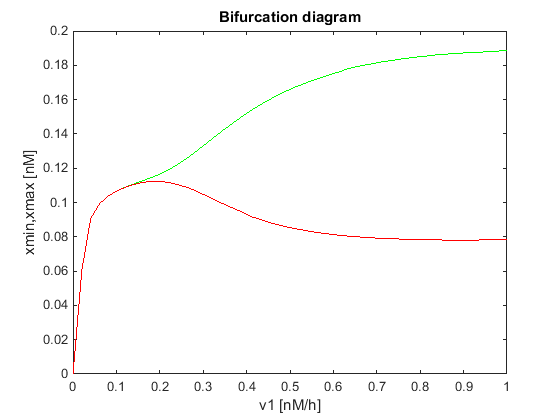
\includegraphics[width=\textwidth]{"../Miniprojet 2.0/Part A/Bifurcation.png}
		\caption{at $t_{max}=1000$ h}
	    \end{subfigure}
	     ~ 
	    \begin{subfigure}[b]{0.35\textwidth}
		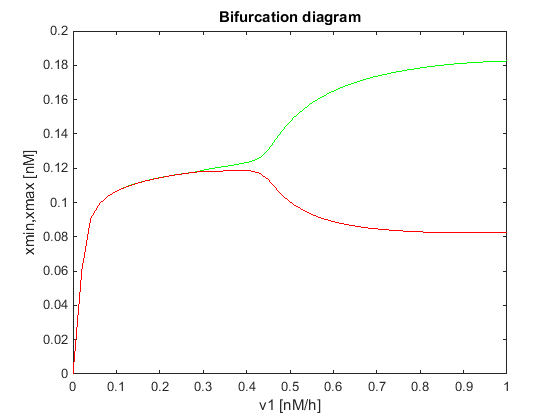
\includegraphics[width=\textwidth]{"../Miniprojet 2.0/Part A/Bifurcation10000.png}
		\caption{at $t_{max}=10~000$ h}
	    \end{subfigure}
	    \caption{\small{Bifurcation Diagram : \red{$X_{min}$} and \green{$X_{max}$} plotted at time intervals $[9/10; 1]$ of $t_{max}$, meaning it plots the maximum and minimum values in the last tenth of the simulation where we are sure that a either a limit cycle or a stable fixed point has already been reached. A limit cycle might be reached when $X_{min} \neq X_{max}$. However, the system needs to be run for enough time for the cycle to be reached, as the (a) suggests. In figure (b) the simulation was run for ten times longer, showing that for values of $v_1$ between 0.2 and 0.4 nM/h, there is very slow oscillatory convergence to a fixed point, which is the same result that is suggested by figure 4 above. The threshold for $v_1$ for the system to reach circadian oscillation seems to be around 0.4 nM/h}}
    \end{figure*}

    \begin{figure*}
    \centering
	\begin{subfigure}[b]{0.32\textwidth}
	    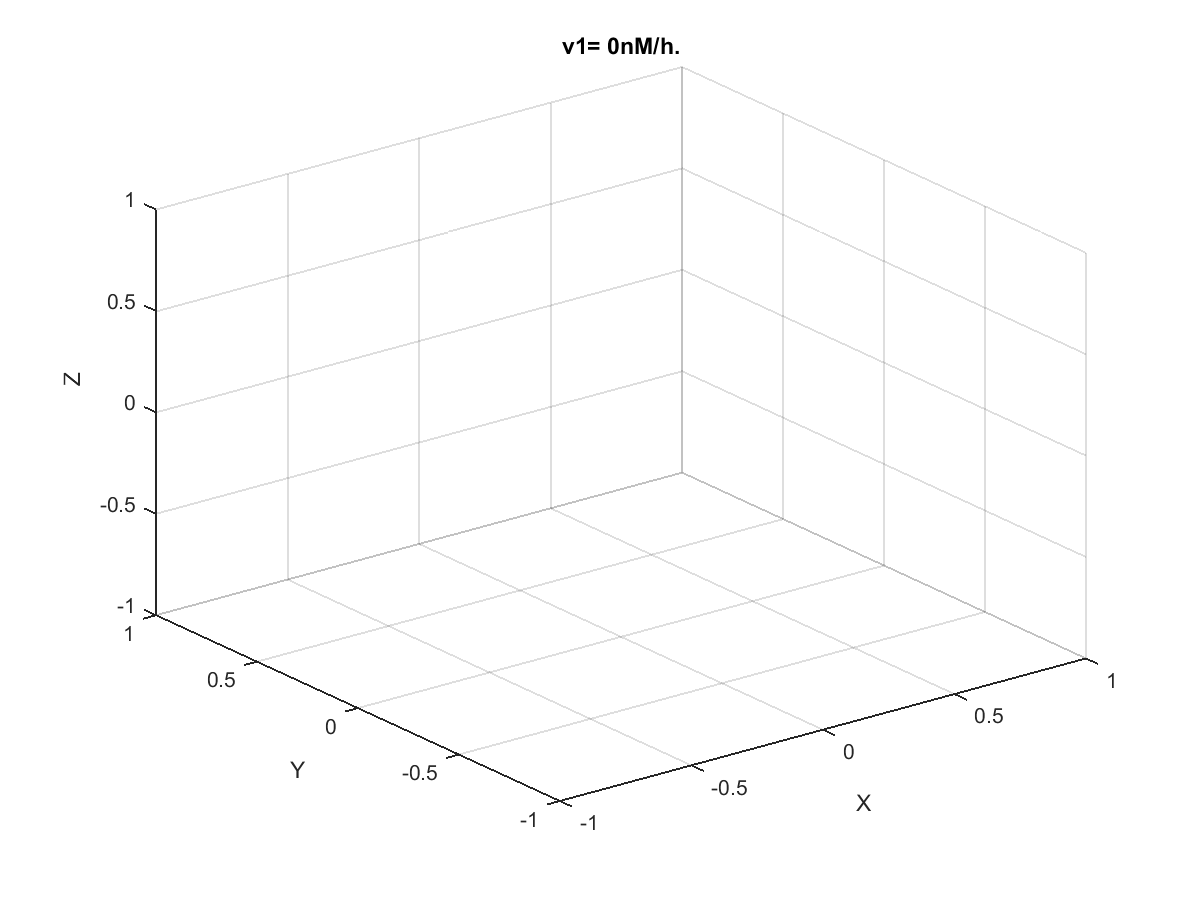
\includegraphics[width=\textwidth]{"../Miniprojet 2.0/Part A/A_3_graphs/A-AA0.png}
	    \caption{$v_1$ = 0 nM/h}
	\end{subfigure}
	~ 
	\begin{subfigure}[b]{0.32\textwidth}
	    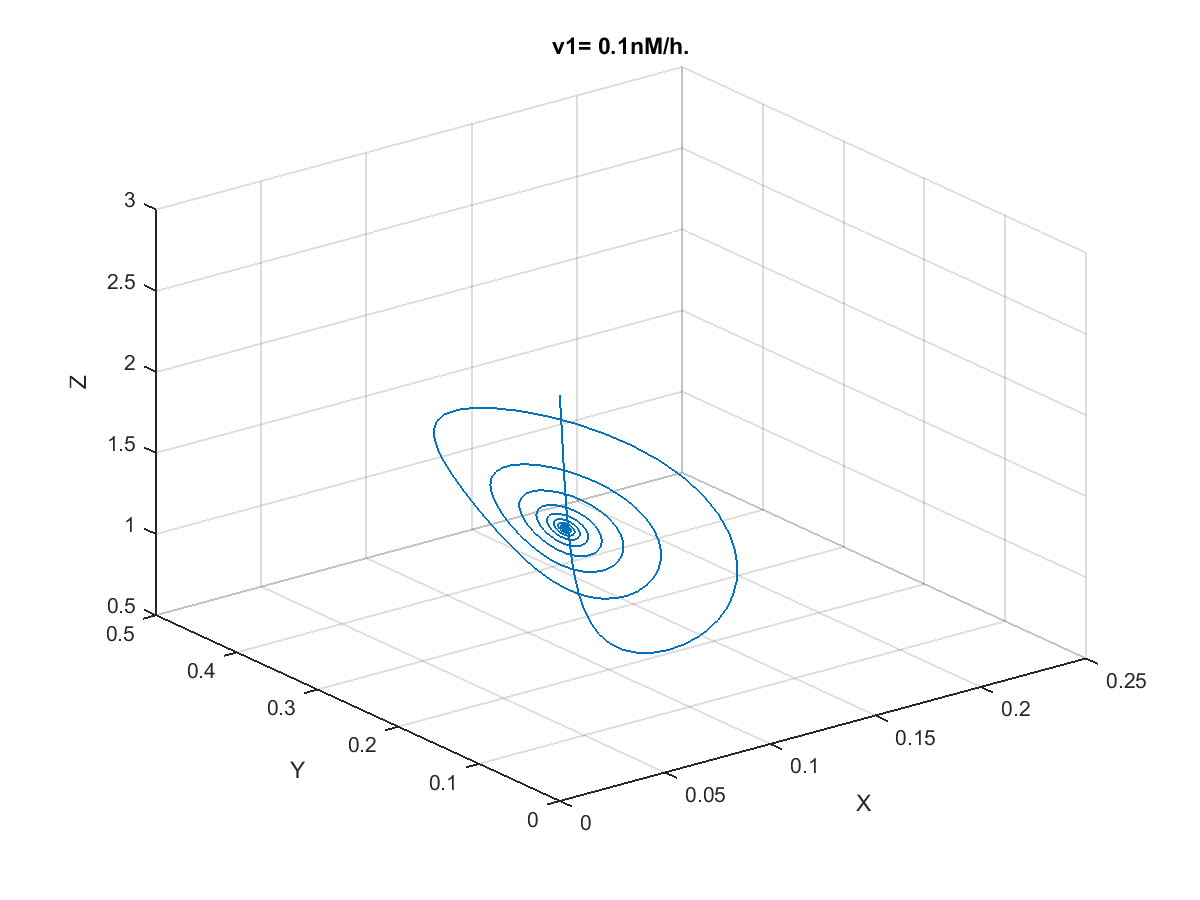
\includegraphics[width=\textwidth]{"../Miniprojet 2.0/Part A/A_3_graphs/A-AA1.png}
	    \caption{$v_1$ = 0.1 nM/h}
	\end{subfigure}
	~ 
	\begin{subfigure}[b]{0.32\textwidth}
	    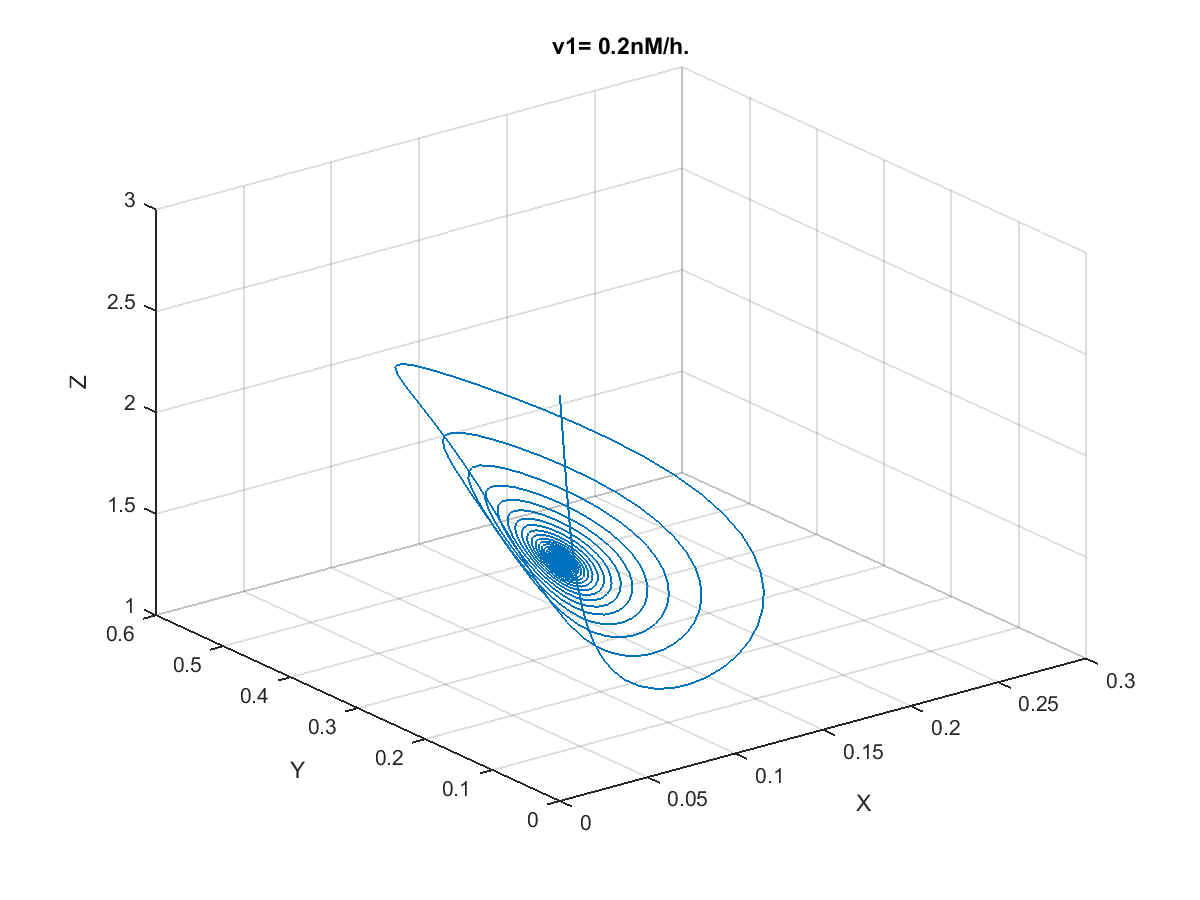
\includegraphics[width=\textwidth]{"../Miniprojet 2.0/Part A/A_3_graphs/A-AA2.png}
	    \caption{$v_1$ = 0.2 nM/h}
	\end{subfigure}
	 
	\begin{subfigure}[b]{0.32\textwidth}
	    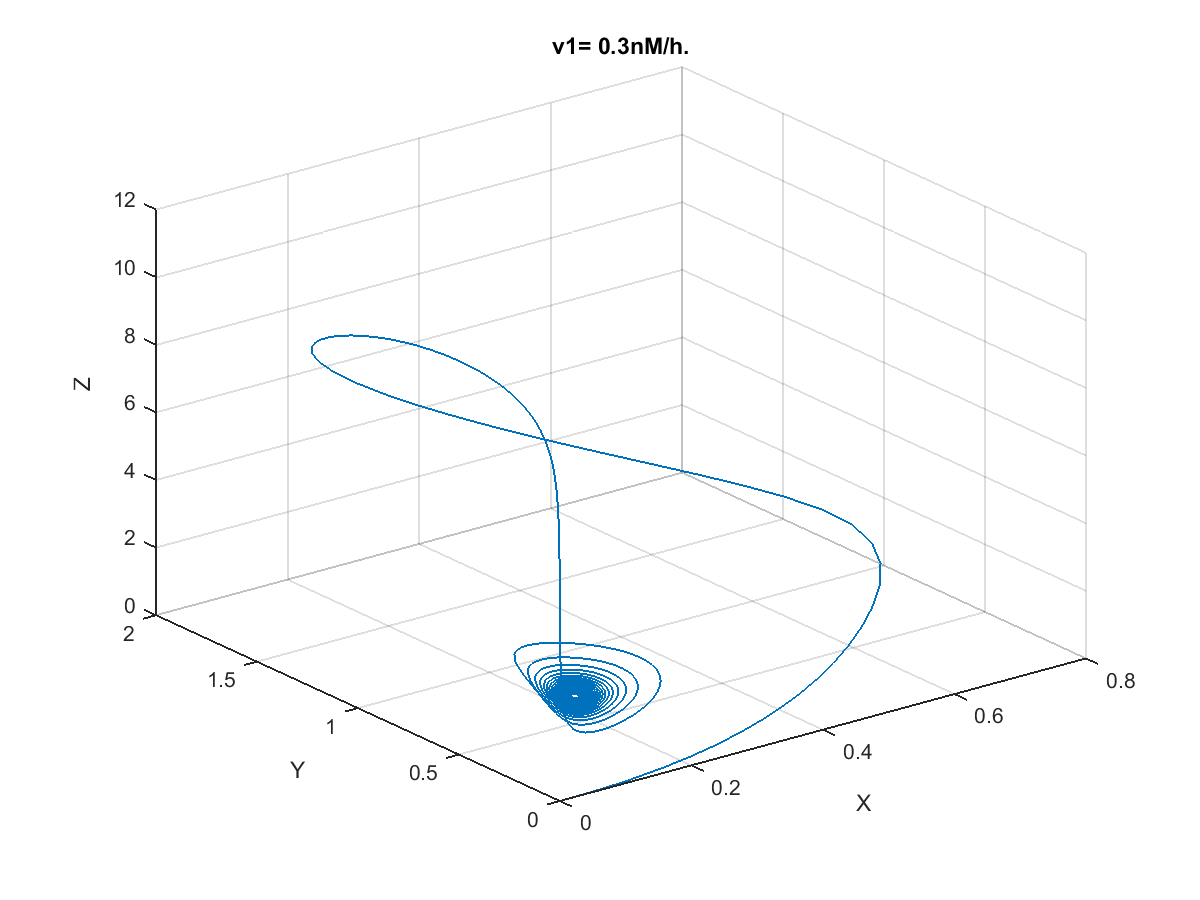
\includegraphics[width=\textwidth]{"../Miniprojet 2.0/Part A/A_3_graphs/A-AA3.png}
	    \caption{$v_1$ = 0.3 nM/h}
	\end{subfigure}
	~ 
	\begin{subfigure}[b]{0.32\textwidth}
	    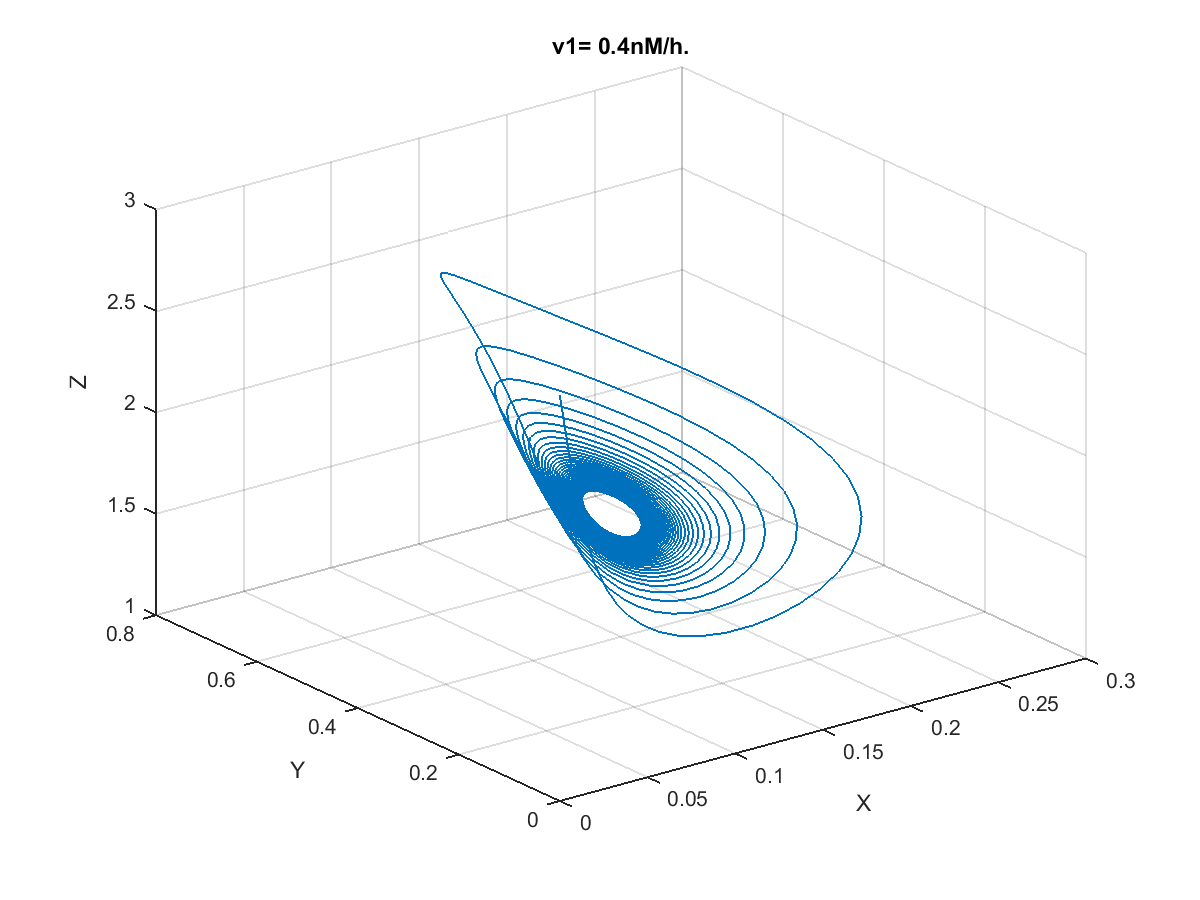
\includegraphics[width=\textwidth]{"../Miniprojet 2.0/Part A/A_3_graphs/A-AA4.png}
	    \caption{$v_1$ = 0.4 nM/h}
	\end{subfigure}
	~
	\begin{subfigure}[b]{0.32\textwidth}
	    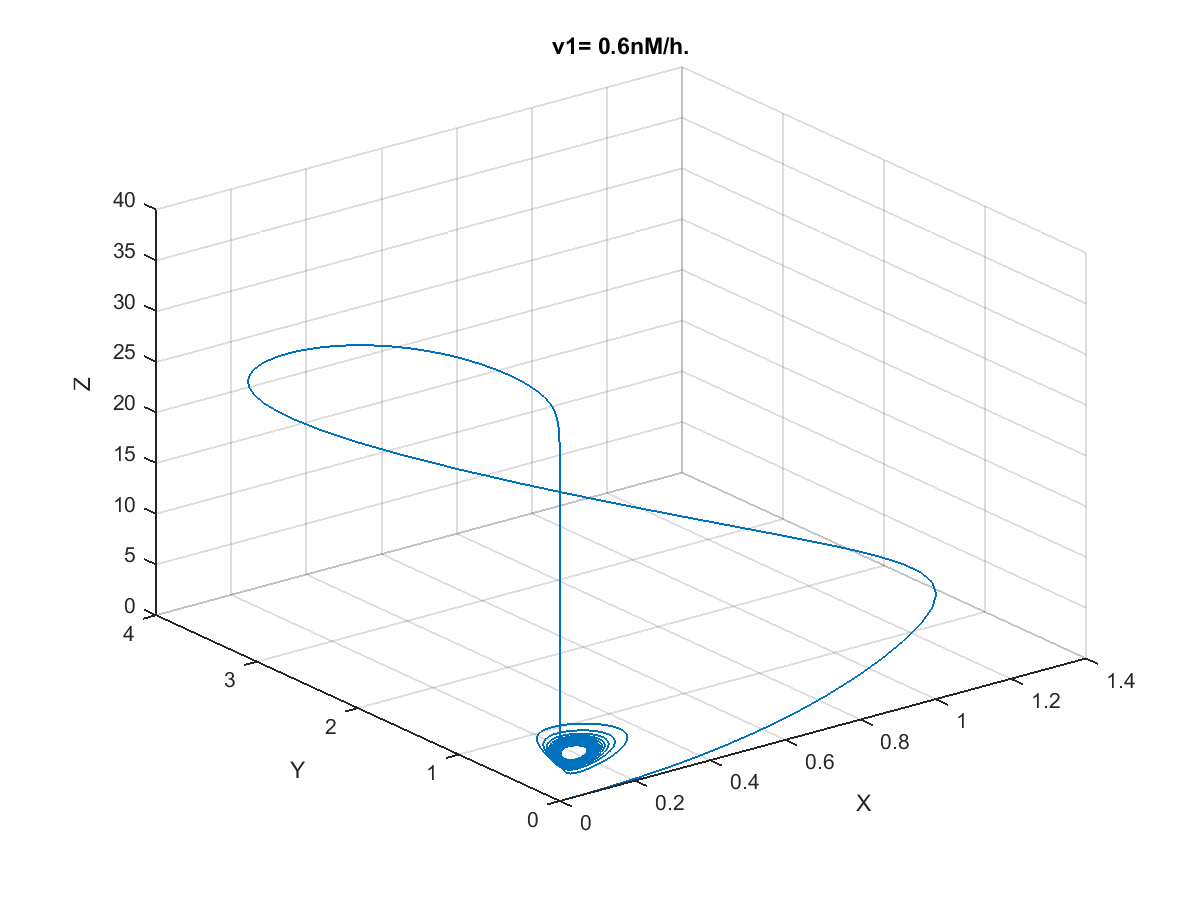
\includegraphics[width=\textwidth]{"../Miniprojet 2.0/Part A/A_3_graphs/A-AA6.png}
	    \caption{$v_1$ = 0.6 nM/h}
	\end{subfigure}
	~ 
	\begin{subfigure}[b]{0.32\textwidth}
	    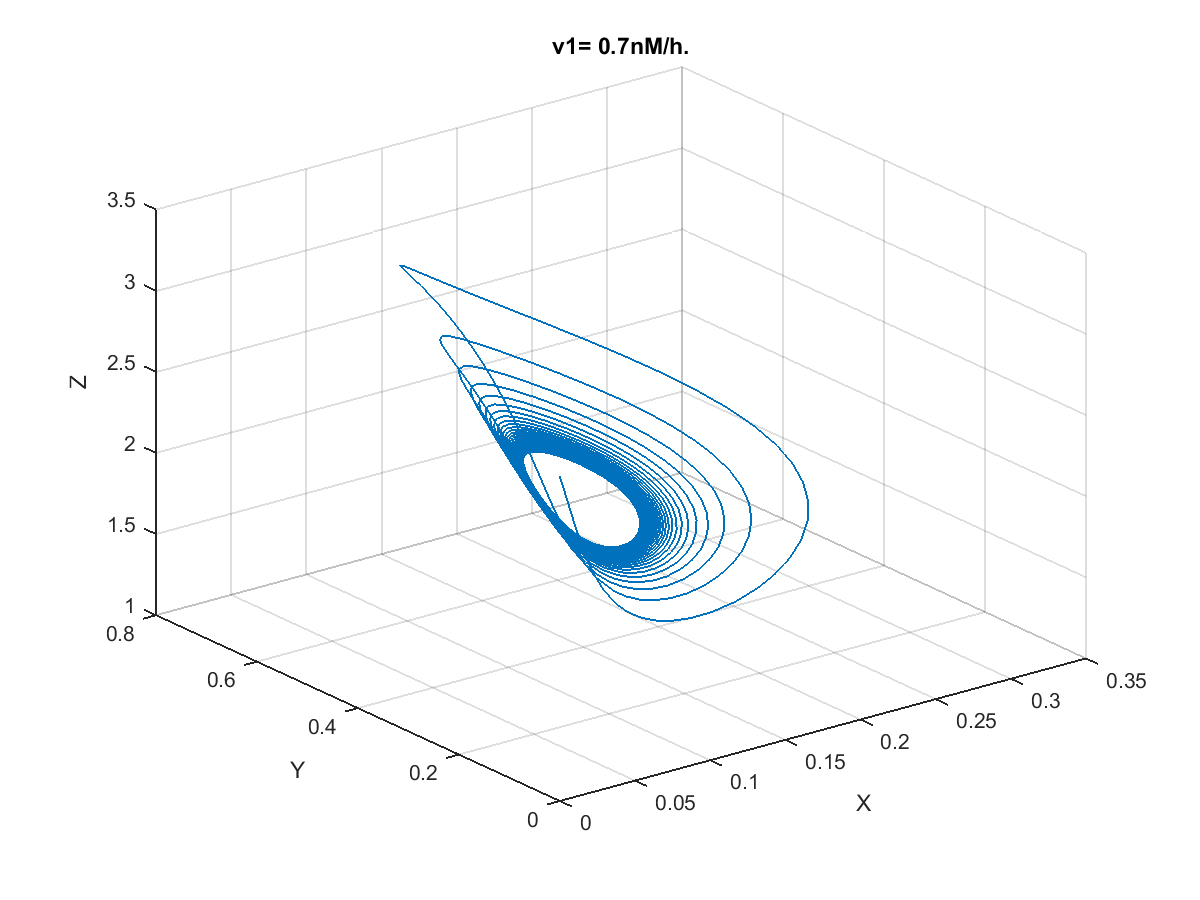
\includegraphics[width=\textwidth]{"../Miniprojet 2.0/Part A/A_3_graphs/A-AA7.png}
	    \caption{$v_1$ = 0.8 nM/h}
	\end{subfigure}
	~
	\begin{subfigure}[b]{0.32\textwidth}
	    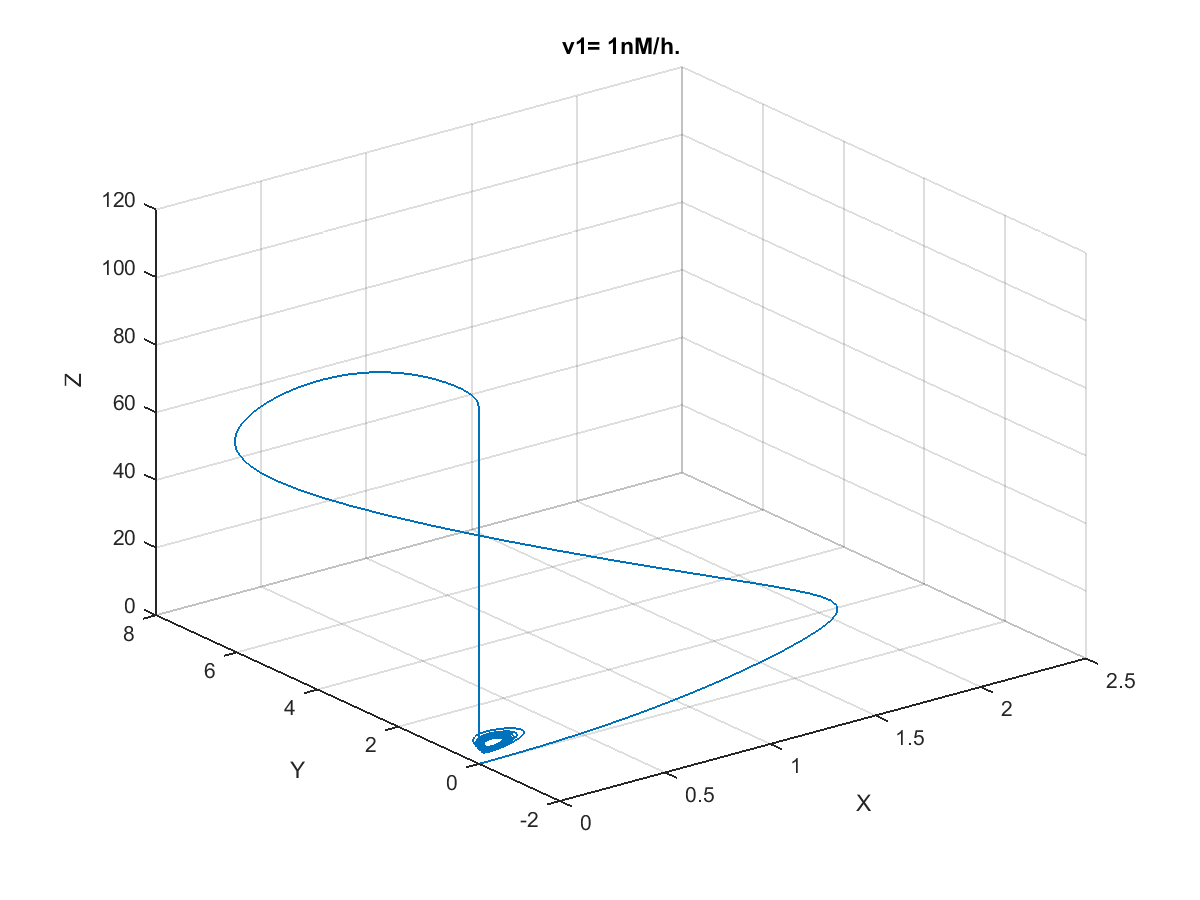
\includegraphics[width=\textwidth]{"../Miniprojet 2.0/Part A/A_3_graphs/A-AA10.png}
	    \caption{$v_1$ = 1 nM/h}
	\end{subfigure}
	
	\caption{Trajectories when varying $v_1$ with initial conditions $X_0 = 0.16$, $Y_0 = 0.33 $, $Z_0 = 1.8$ [nM]\\
	$v_1$ has to reach a certain value for $X(t)$ to be able to compensate its inhibition by $Z(t)$ and therefore for the system to reach a limit cycle. We observe that this value is around 0.4 nM/h, as the trajectories still converge close to zero in (e); there is an 'eye', even though it is smaller than in (f) and (g). It is possible that the simulation time is not long enough to let the system dissipate completely.
	}
	\label{fig:6}
    \end{figure*}

    \begin{figure*}
	\centering
	\begin{subfigure}[b]{0.4\textwidth}
	    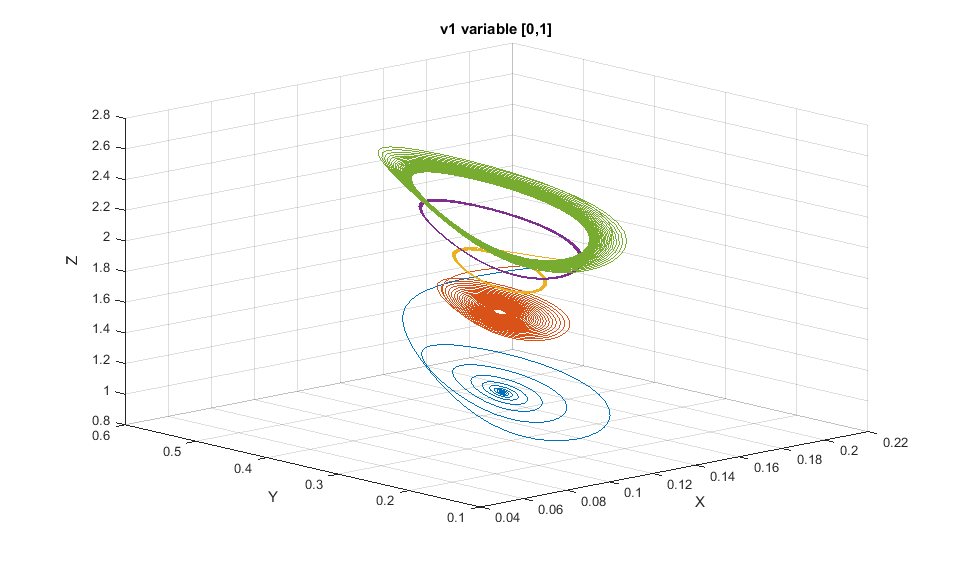
\includegraphics[width=\textwidth]{"../Miniprojet 2.0/Part A/A2.png}
	    \caption{Superimposed trajectories at late timepoints with initial conditions $X_0 = 0.16$, $Y_0 = 0.33 $, $Z_0 = 1.8$ [nM] and $v_1$ = \cyan{0.1}/\red{0.3}/\orange{0.5}/\purple{0.7}/\fgreen{0.9} nM/h. We observe here that $Z(t)$ tends to reach greater concentration stability with increasing $v_1$.}
	\end{subfigure}
	~
	\begin{subfigure}[b]{0.4\textwidth}
	    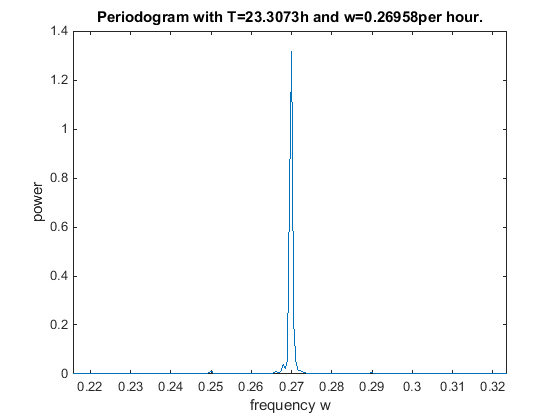
\includegraphics[width=\textwidth]{"../Miniprojet 2.0/Part A/periodogram.png}
	    \caption{Periodogram of the oscillations above with \\ $v_1$ =0.7nM/h.}
	\end{subfigure}
	\caption{This analysis of the trajectories allows to sample for frequencies that are strongly represented in a set of data points. The simulations above appear to have a strong representation around a frequency that corresponds to a period of 23.4 hours, which is close to the 24 hour circadian rhythm that is observed in nature.}
    \end{figure*}

    \begin{figure*}[!htb] 		%oh my god this is so ugly pls don't look at me
	\captionsetup{labelformat=empty}
	\caption{\Huge{\textbf{Part B - Multiple Cells Model}}}
    \end{figure*}

    \begin{figure*}[!h]
	\begin{subfigure}[b]{0.5\textwidth}
	    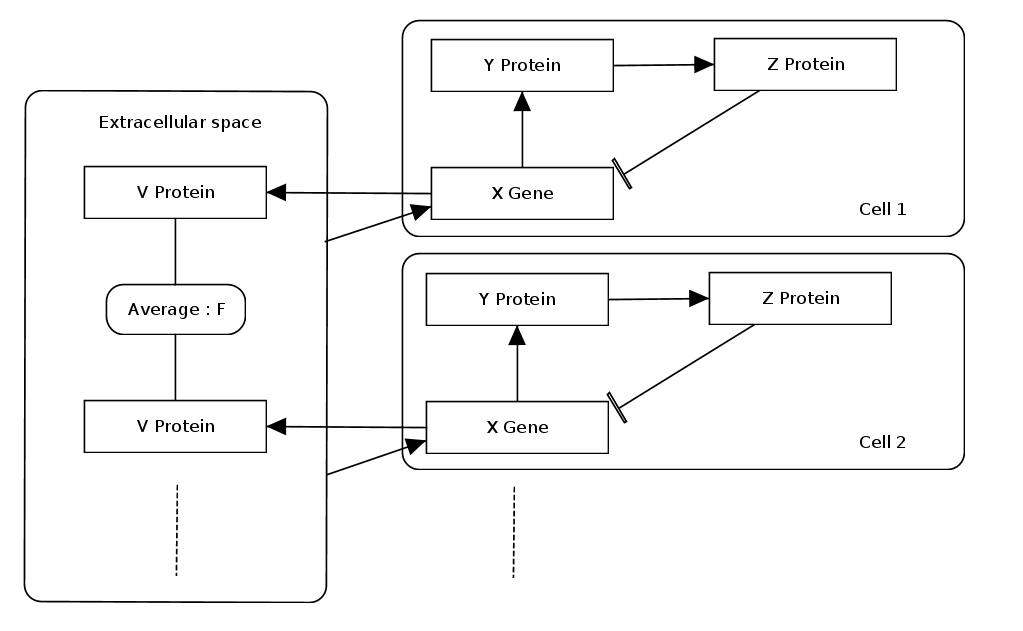
\includegraphics[width=\textwidth]{sketch2.png}
	    \caption{
		Multiple Cells Model\\
	    The gene $X$ codes for protein $Y$ which, in turn, activates transcriptional inhibitor $Z$. In addition, gene $X$ activates a positive feedback loop through the mean concentration of extracellular protein $V$
	    }
	\end{subfigure}
	~
	\begin{subfigure}[b]{0.5\textwidth}
	    \begin{equation*}\frac{\delta X}{\delta t} = v_1 \frac{K_1^n}{K_1^n + Z^n} - v_2 \frac{X}{K_2 + X} + v_c\frac{KF}{K_c + KF}\end{equation*}
	    \begin{equation*}\frac{\delta Y}{\delta t} = k_3 X - v_4 \frac{Y}{K_4 + Y}\end{equation*}
	    \begin{equation*}\frac{\delta Z}{\delta t} = k_5 Y - v_6 \frac{Z}{K_6 + Z}\end{equation*}
	    \begin{equation*}\frac{\delta V_i}{\delta t} = k_7 X_i - v_8 \frac{V_i}{K_8 + V_i}\end{equation*}
	    \begin{equation*}\text{where } F = \frac{1}{N}\sum_{i=1}^{N}V_i\end{equation*}

	    \captionsetup{labelformat=empty}
	    \caption{\\
	    \begin{tabular}{@{}>{$}l<{$}l @{\hskip 0.2cm} | @{\hskip 0.2cm} @{}>{$}l<{$}l@{}}
		v_1 & translation rate of $X$ & k_1 & transcription rate of $X$ \\
		v_2 & degradation rate of $X$ &	K_1 & Michaelis constant of $X$ \\
		v_4 & degradation rate of $Y$ & K_4 & Michaelis constant of $Y$ \\
		v_6 & degradation rate of $Z$ & K_6 & Michaelis constant of $Z$ \\
		v_8 & degradation rate of $V$ & K_8 & Michaelis constant of $V$ \\
		k_3 & transcription rate of $Y$ & K_c & Michaelis constant of $X$ by $F$\\
		k_5 & transcription rate of $Z$ & v_c & Activation rate of $X$ by $F$ \\
		k_7 & transcription rate of $V$ & K & Coupling Constant \\
	    \end{tabular}
	    }
	\end{subfigure}
    \end{figure*}

    \begin{figure*}
    \centering
	\begin{subfigure}[b]{0.32\textwidth}
	    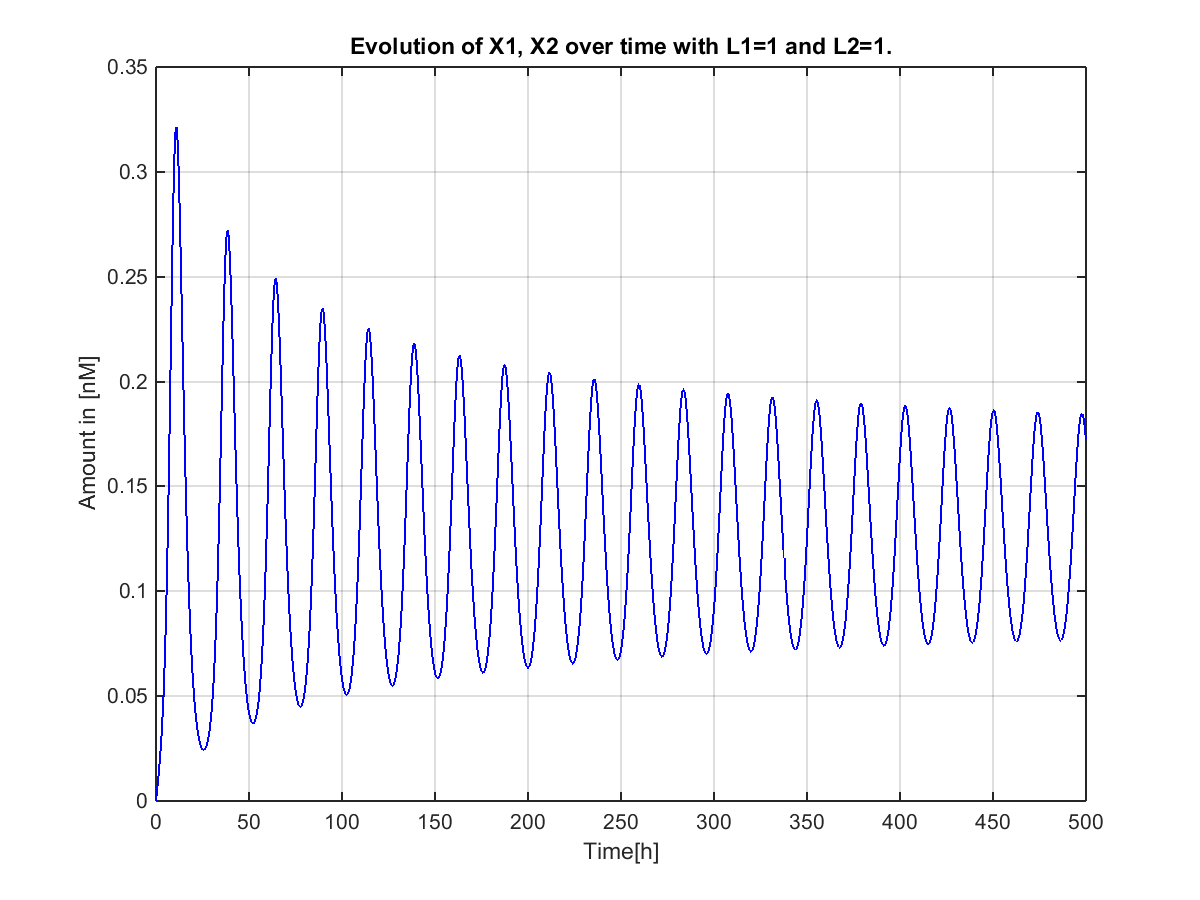
\includegraphics[width=\textwidth]{"../Miniprojet 2.0/Part B/B_2_graphs/B21.png}
	    \caption{$\lambda_1$ = 1, $\lambda_2$ = 1 [$h^{-1}$]}
	\end{subfigure}
	~ 
	\begin{subfigure}[b]{0.32\textwidth}
	    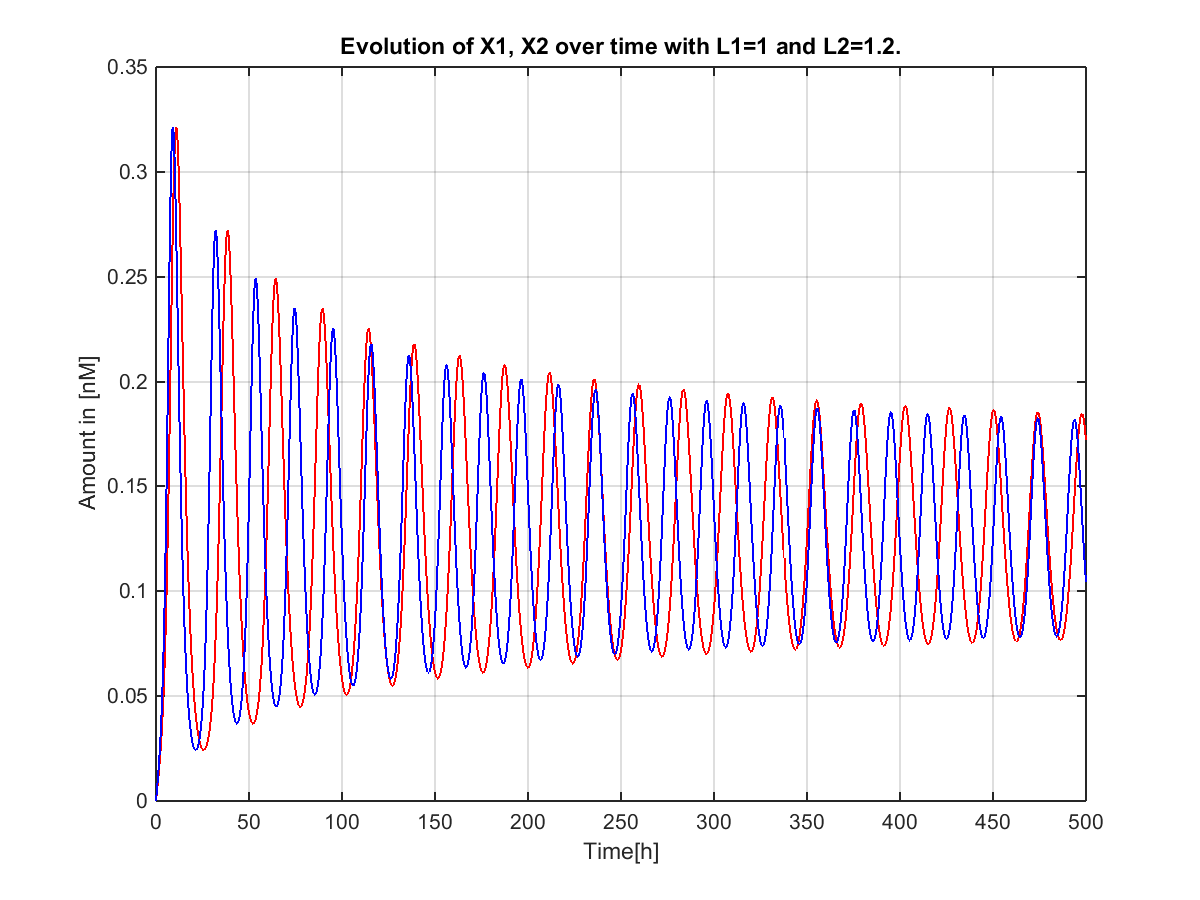
\includegraphics[width=\textwidth]{"../Miniprojet 2.0/Part B/B_2_graphs/B22.png}
	    \caption{$\lambda_1$ = 1, $\lambda_2$ = 1.2 [$h^{-1}$]}
	\end{subfigure}
	~ 
	\begin{subfigure}[b]{0.32\textwidth}
	    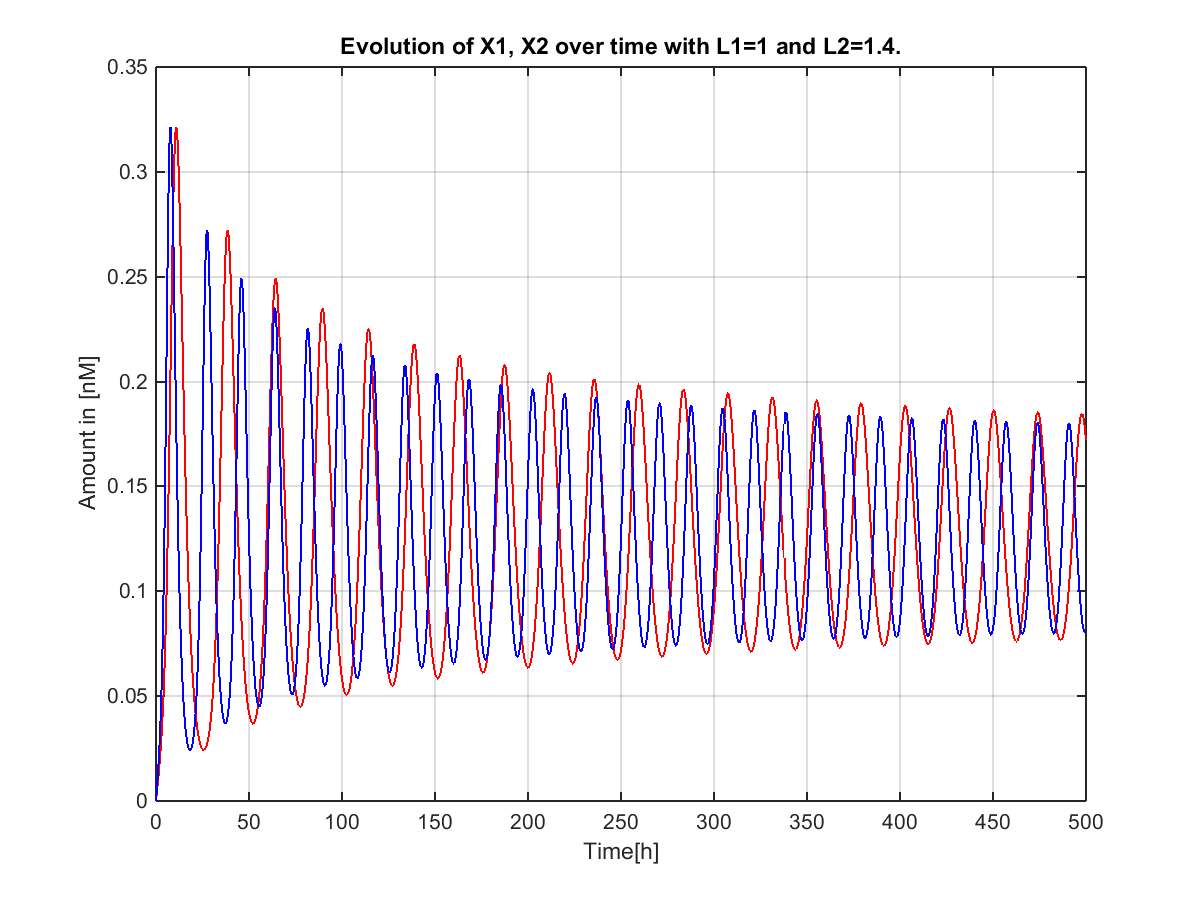
\includegraphics[width=\textwidth]{"../Miniprojet 2.0/Part B/B_2_graphs/B23.png}
	    \caption{$\lambda_1$ = 1, $\lambda_2$ = 1.4 [$h^{-1}$]}
	\end{subfigure}
	 
	\begin{subfigure}[b]{0.32\textwidth}
	    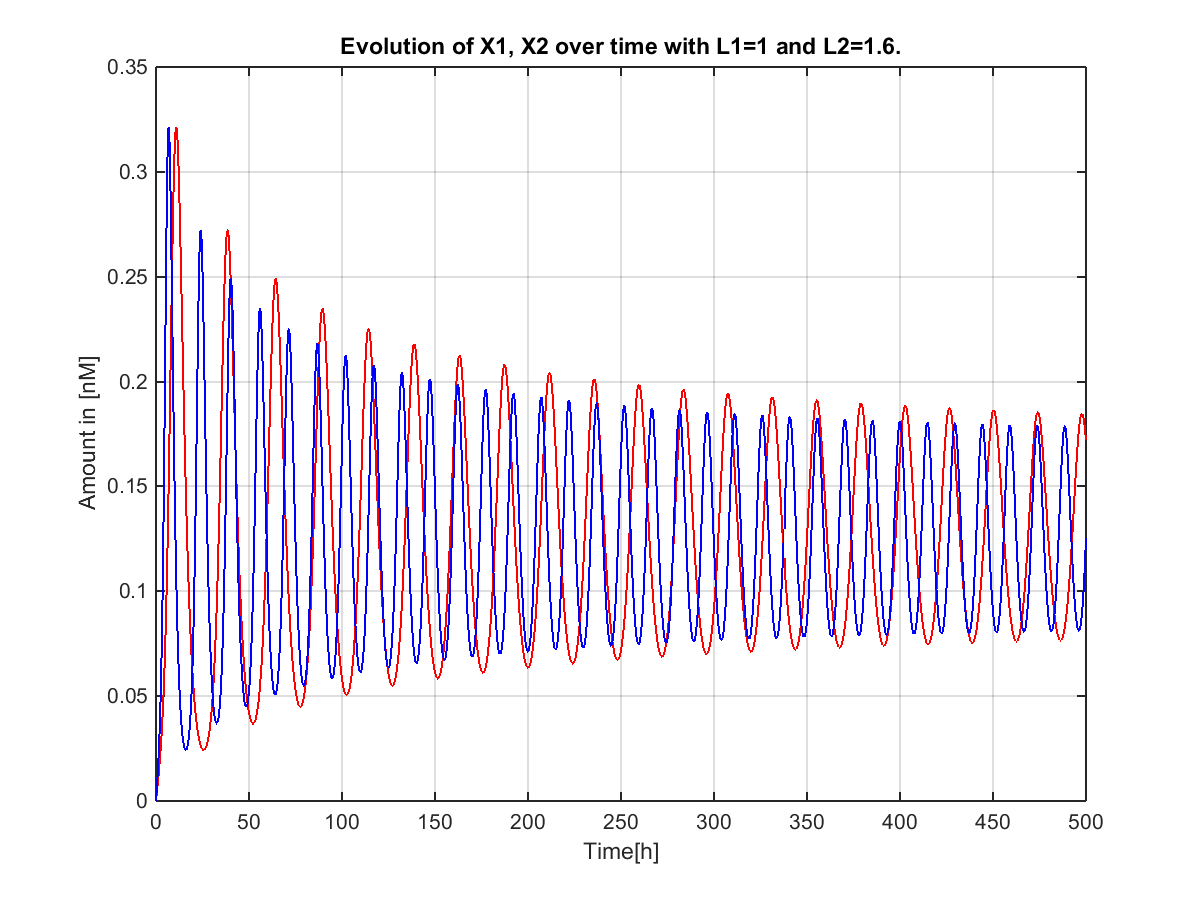
\includegraphics[width=\textwidth]{"../Miniprojet 2.0/Part B/B_2_graphs/B24.png}
	    \caption{$\lambda_1$ = 1, $\lambda_2$ = 1.6 [$h^{-1}$]}
	\end{subfigure}
	~ 
	\begin{subfigure}[b]{0.32\textwidth}
	    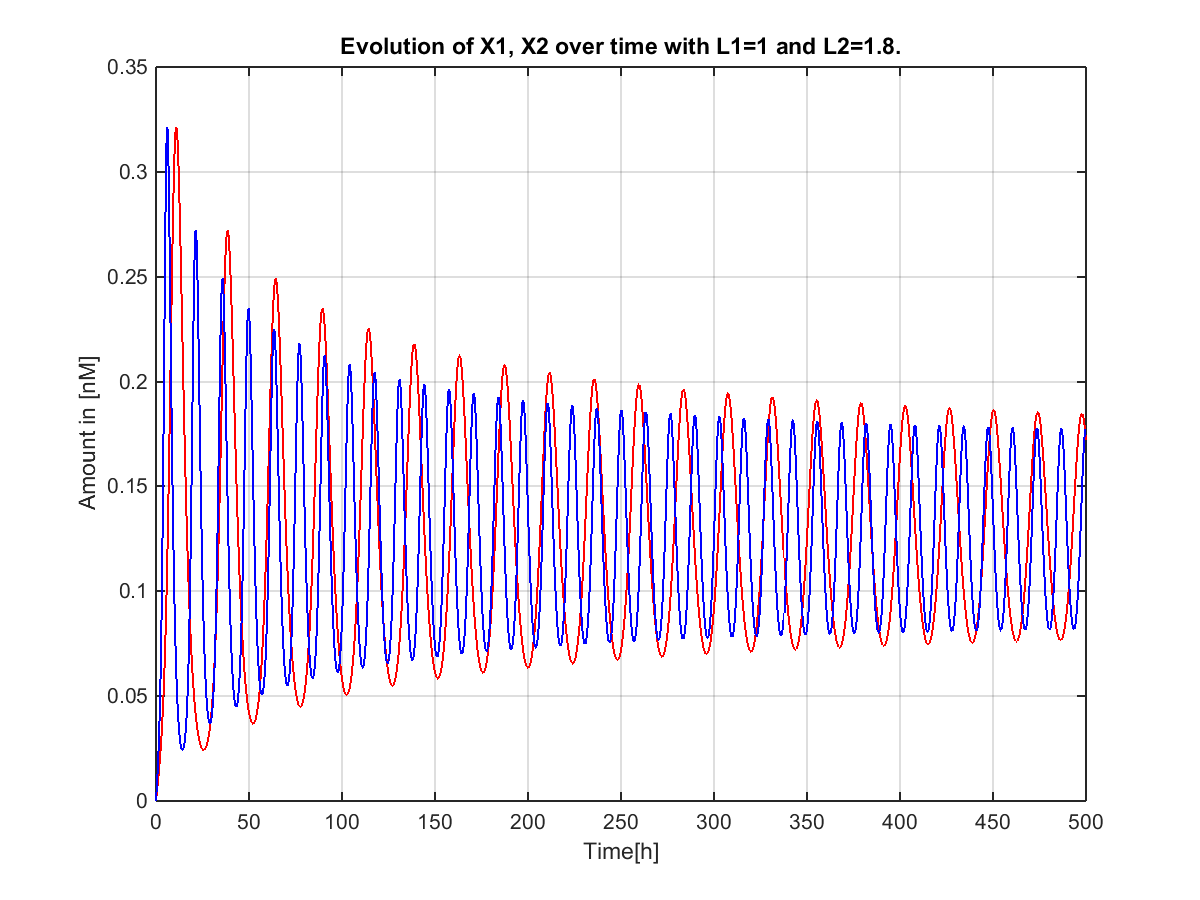
\includegraphics[width=\textwidth]{"../Miniprojet 2.0/Part B/B_2_graphs/B25.png}
	    \caption{$\lambda_1$ = 1, $\lambda_2$ = 1.8 [$h^{-1}$]}
	\end{subfigure}
	~ 
	\begin{subfigure}[b]{0.32\textwidth}
	    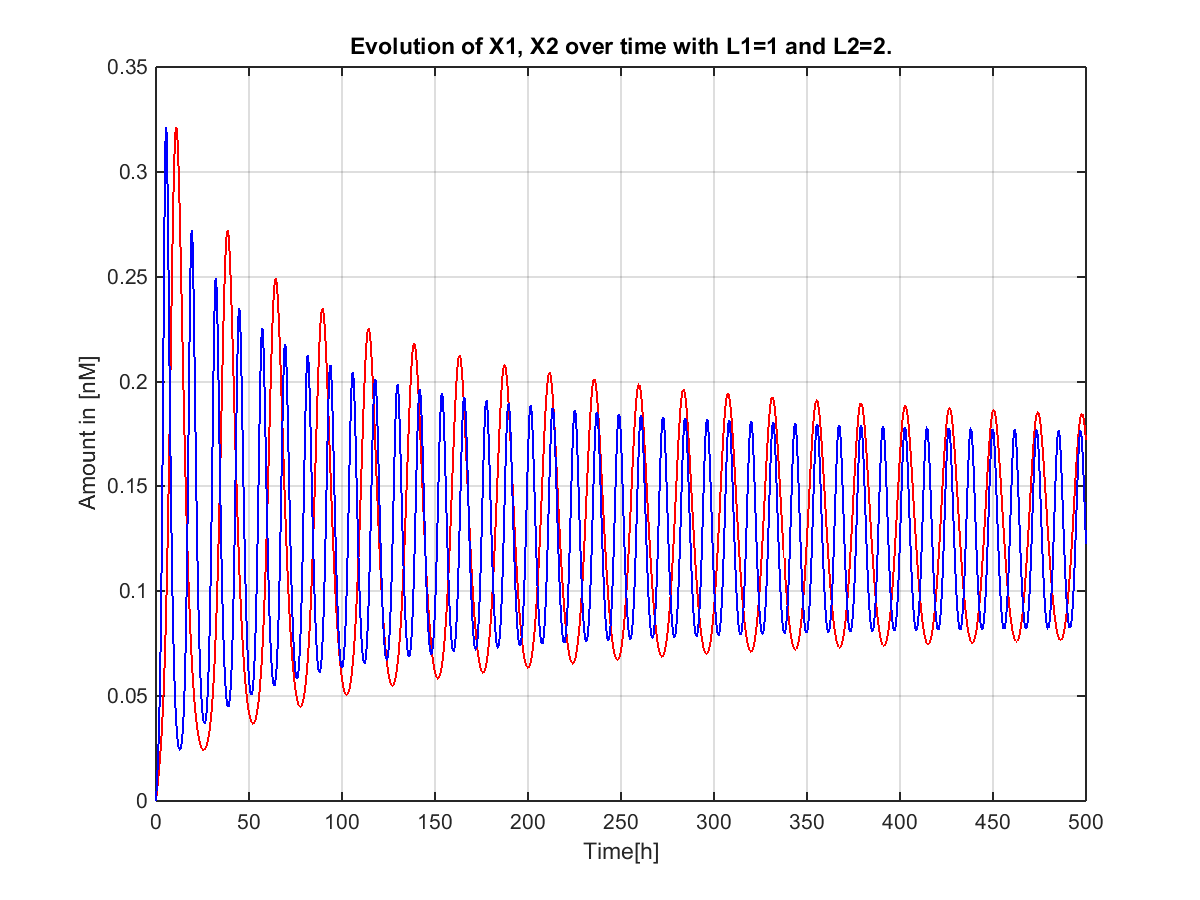
\includegraphics[width=\textwidth]{"../Miniprojet 2.0/Part B/B_2_graphs/B26.png}
	    \caption{$\lambda_1$ = 1, $\lambda_2$ = 2 [$h^{-1}$]}
	\end{subfigure}

	\caption{\red{$X_1(t)$} and \blue{$X_2(t)$} trajectories in a two-cells Model with $K=0$ ($\leftrightarrow$ no coupling)\\
	Figure (a) has both signals perfectly aligned. We observe no synchronisation, as expected These figures mainly serve to show whether the signals are in or out of phase, to help interpret figure 11 more easily.}
    \end{figure*}


    \begin{figure*}
    \centering
	\begin{subfigure}[b]{0.32\textwidth}
	    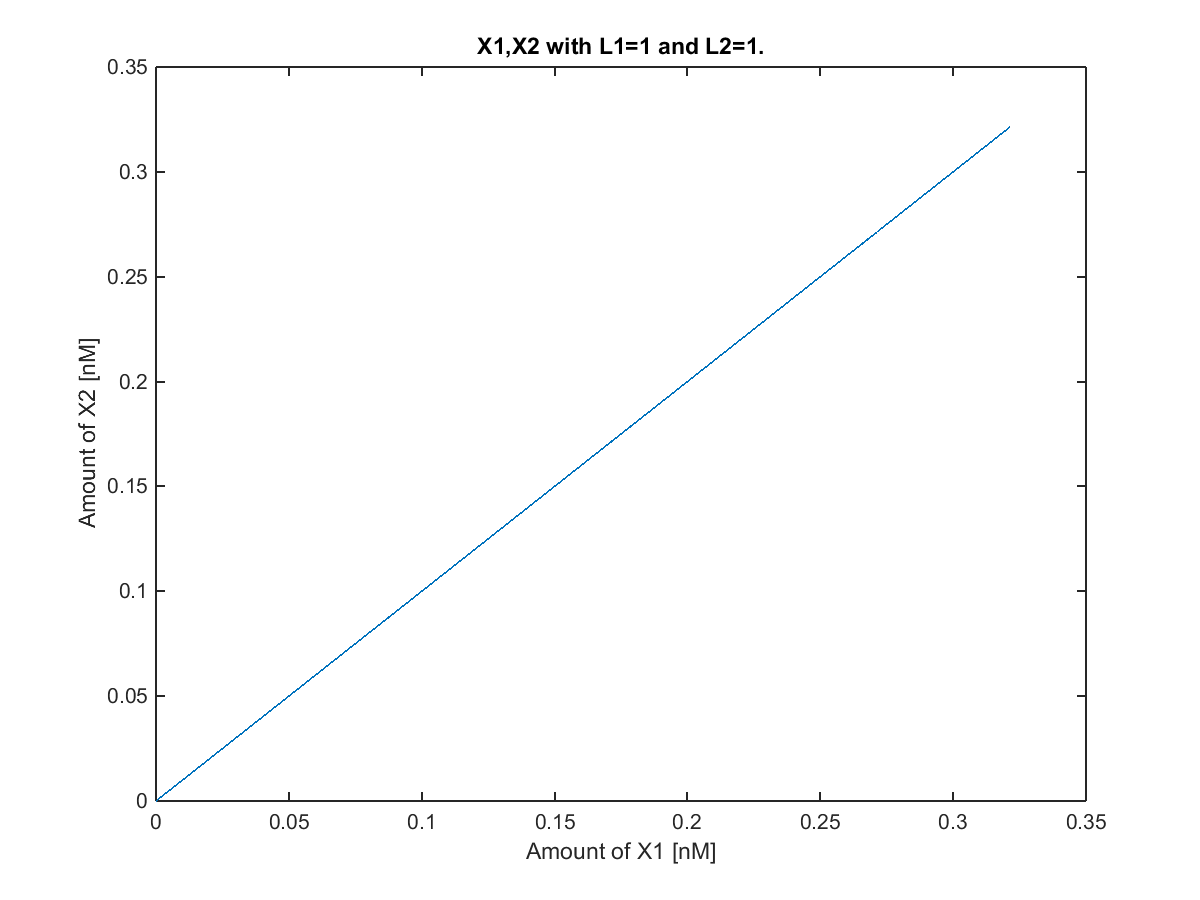
\includegraphics[width=\textwidth]{"../Miniprojet 2.0/Part B/B_2_graphs/B11.png}
	    \caption{$\lambda_1$ = 1, $\lambda_2$ = 1 [$h^{-1}$]}
	\end{subfigure}
	~ 
	\begin{subfigure}[b]{0.32\textwidth}
	    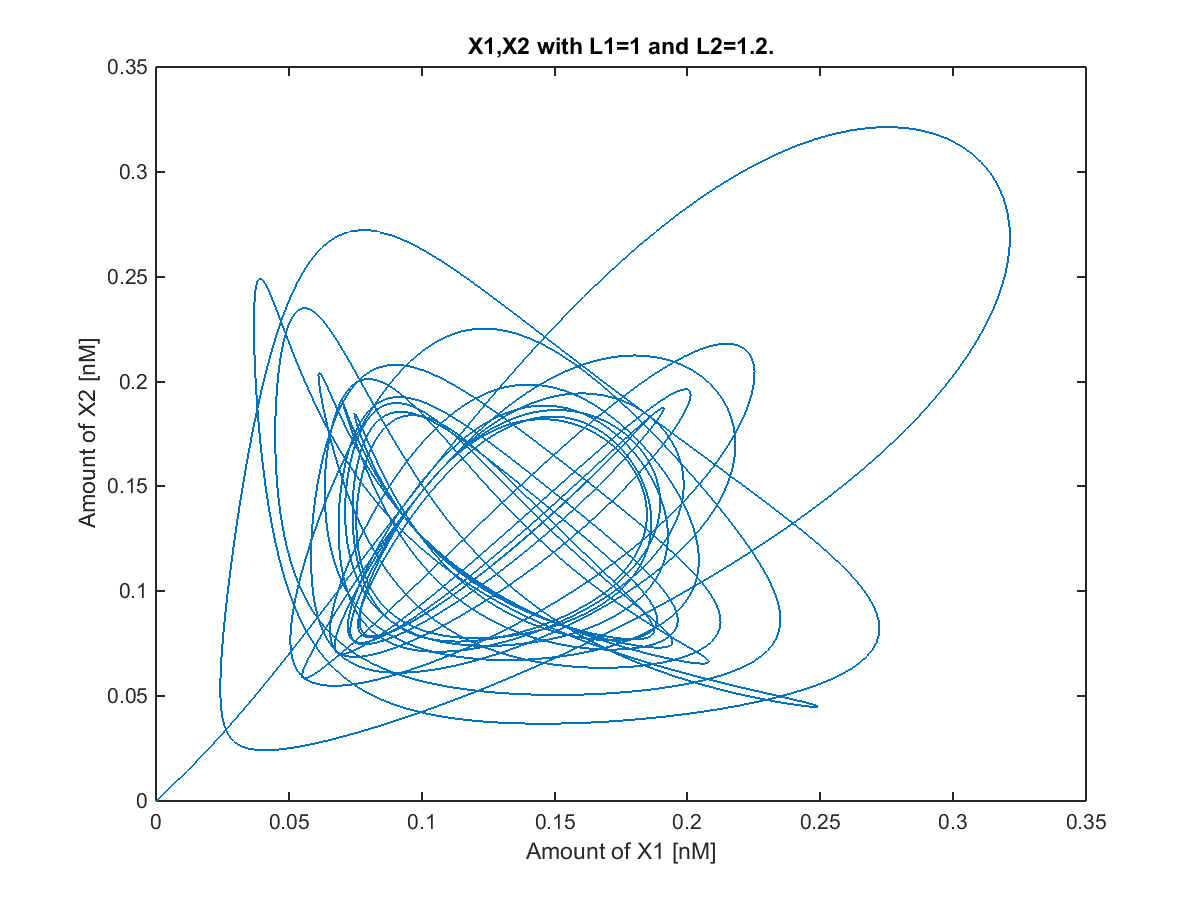
\includegraphics[width=\textwidth]{"../Miniprojet 2.0/Part B/B_2_graphs/B12.png}
	    \caption{$\lambda_1$ = 1, $\lambda_2$ = 1.2 [$h^{-1}$]}
	\end{subfigure}
	~ 
	\begin{subfigure}[b]{0.32\textwidth}
	    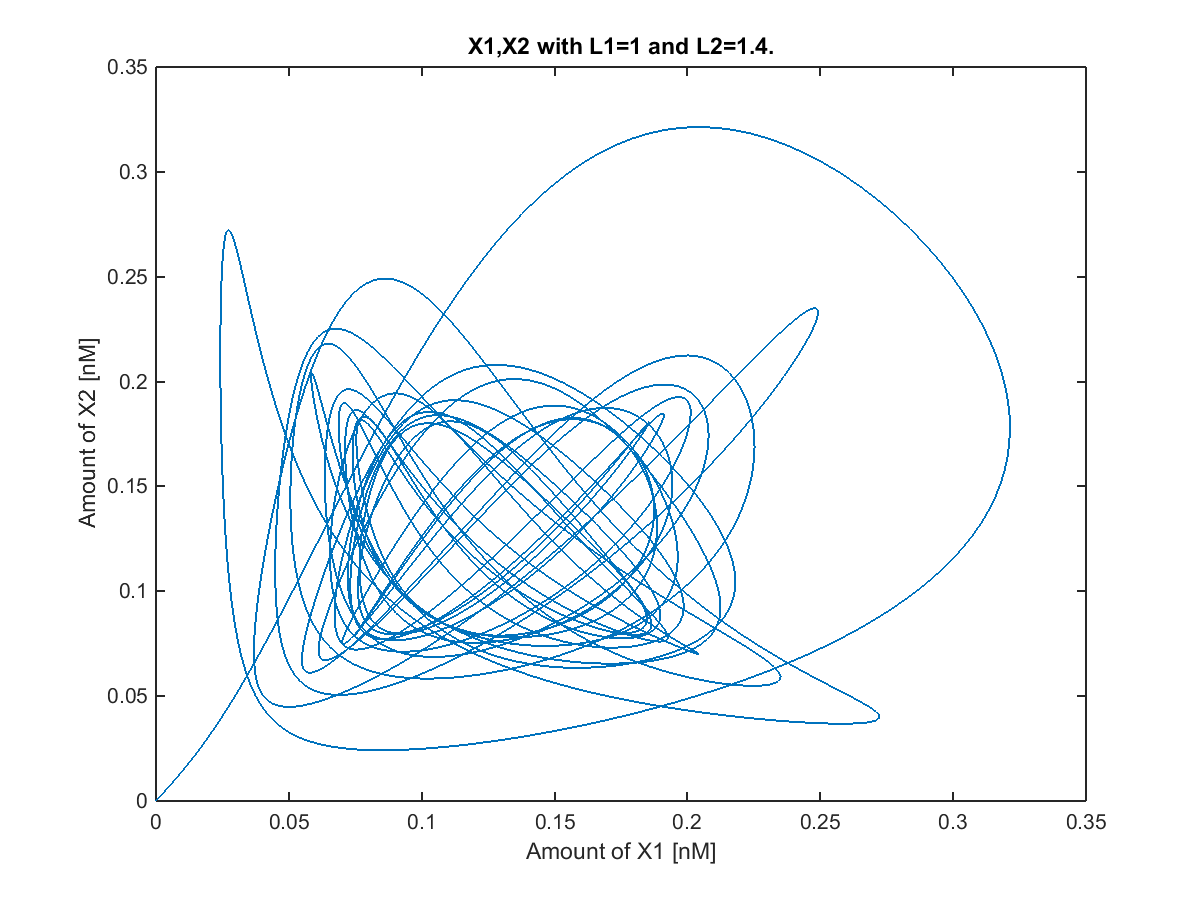
\includegraphics[width=\textwidth]{"../Miniprojet 2.0/Part B/B_2_graphs/B13.png}
	    \caption{$\lambda_1$ = 1, $\lambda_2$ = 1.4 [$h^{-1}$]}
	\end{subfigure}
	 
	\begin{subfigure}[b]{0.32\textwidth}
	    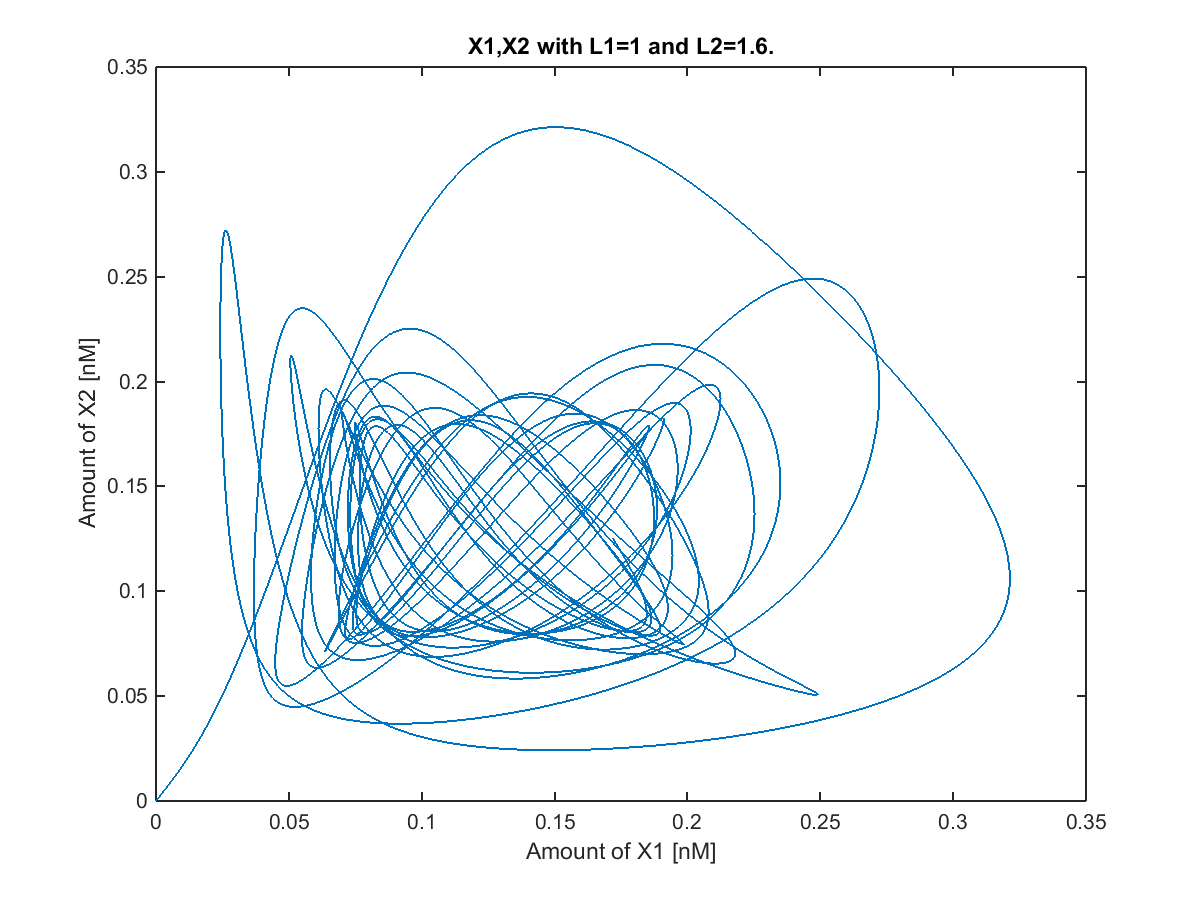
\includegraphics[width=\textwidth]{"../Miniprojet 2.0/Part B/B_2_graphs/B14.png}
	    \caption{$\lambda_1$ = 1, $\lambda_2$ = 1.6 [$h^{-1}$]}
	\end{subfigure}
	~ 
	\begin{subfigure}[b]{0.32\textwidth}
	    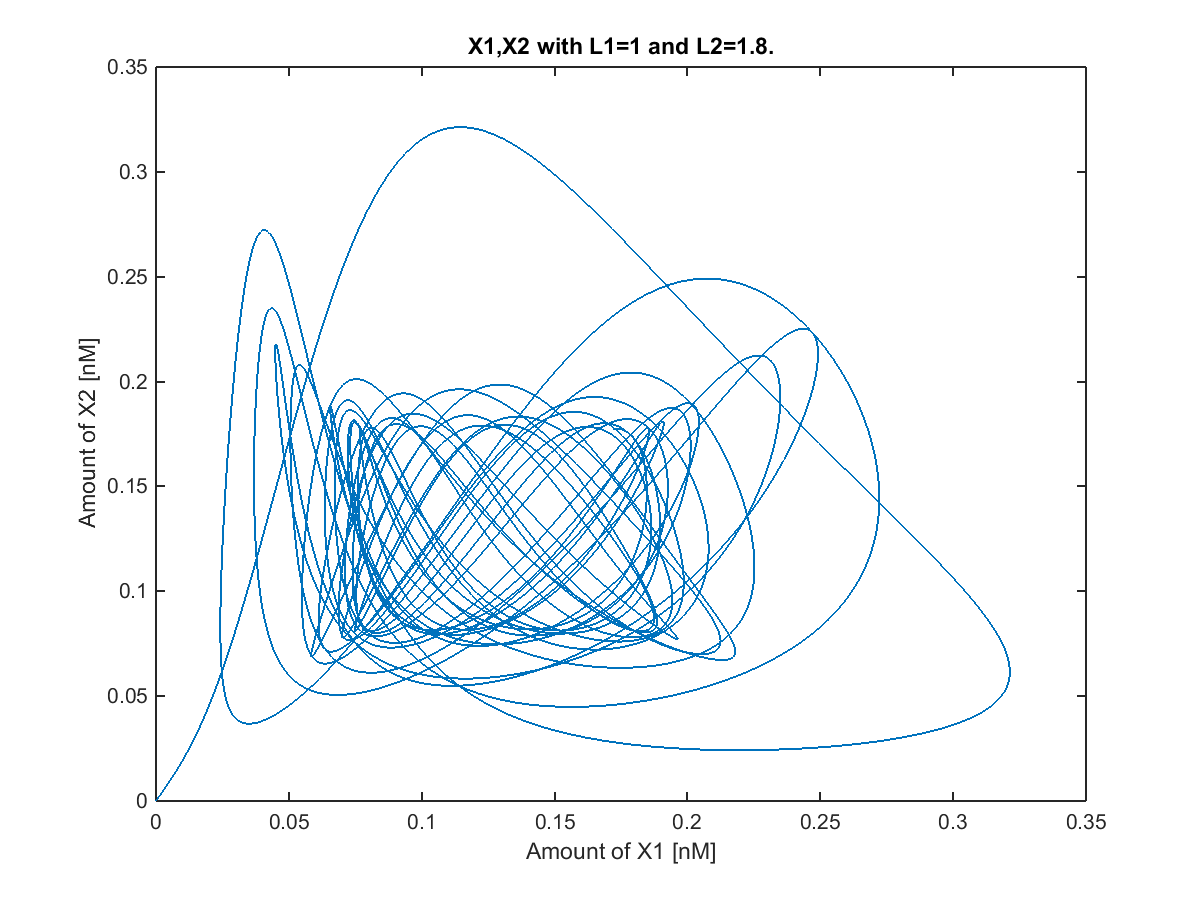
\includegraphics[width=\textwidth]{"../Miniprojet 2.0/Part B/B_2_graphs/B15.png}
	    \caption{$\lambda_1$ = 1, $\lambda_2$ = 1.8 [$h^{-1}$]}
	\end{subfigure}
	~ 
	\begin{subfigure}[b]{0.32\textwidth}
	    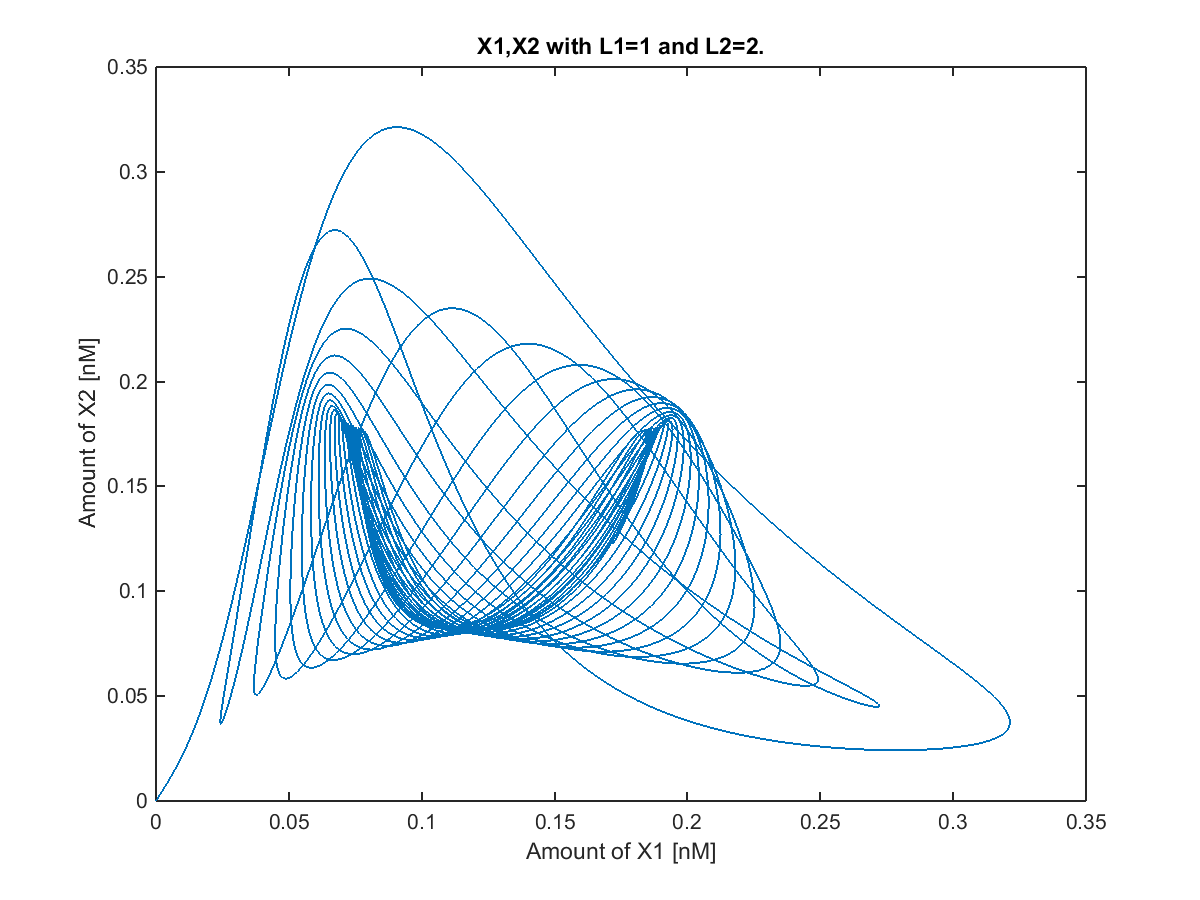
\includegraphics[width=\textwidth]{"../Miniprojet 2.0/Part B/B_2_graphs/B16.png}
	    \caption{$\lambda_1$ = 1, $\lambda_2$ = 2 [$h^{-1}$]}
	\end{subfigure}

	\caption{$X_1$ and $X_2$ trajectories with varying $\lambda_i$ in a two-cells Model with $K=0$\\
	Figure (a), the control, makes perfect sense since the two cells have the same period, hence the exact same signal. With unequal periods, the limit cycles of both cells aren't in phase and form these '8' patterns. The fluctuations at the beginning of trajectories come from the inner adjustment of the cells (see Figure \ref{fig:6}). The sides of the rectangles that appear represent the variation of $X_1$ and $X_2$  between their minimal and maximal values and receiving a rectangle shows us that we reach a limit cycle. (f) gives us a different pattern due to the two periods being a multiple of each other. We expect the phase difference not to vary greatly over time, as in the other figures. }
	\label{fig:11}
    \end{figure*}
    
   \begin{figure*}
    \centering
	\begin{subfigure}[b]{0.32\textwidth}
	    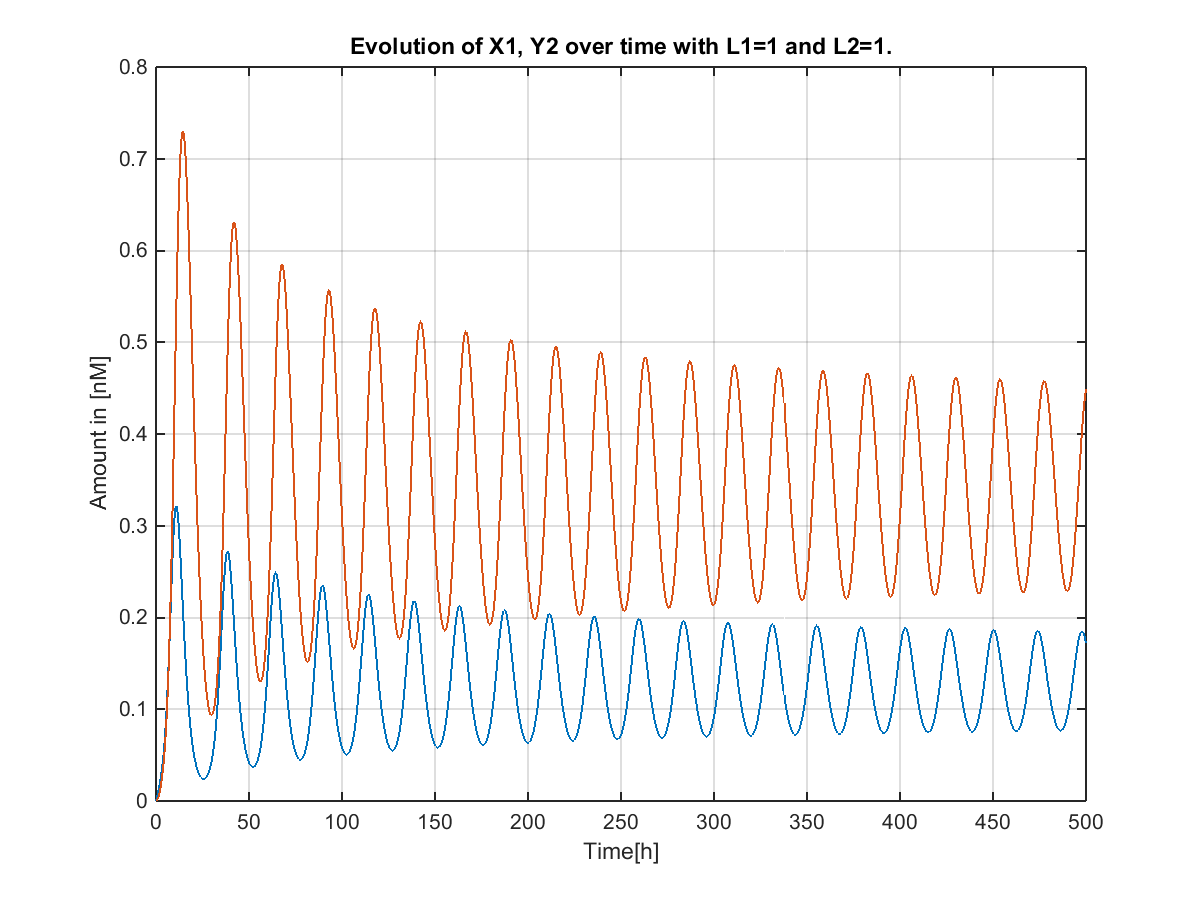
\includegraphics[width=\textwidth]{"../Miniprojet 2.0/Part B/B_2_graphs/B41.png}
	    \caption{$\lambda_1$ = 1, $\lambda_2$ = 1 [$h^{-1}$]}
	\end{subfigure}
	~ 
	\begin{subfigure}[b]{0.32\textwidth}
	    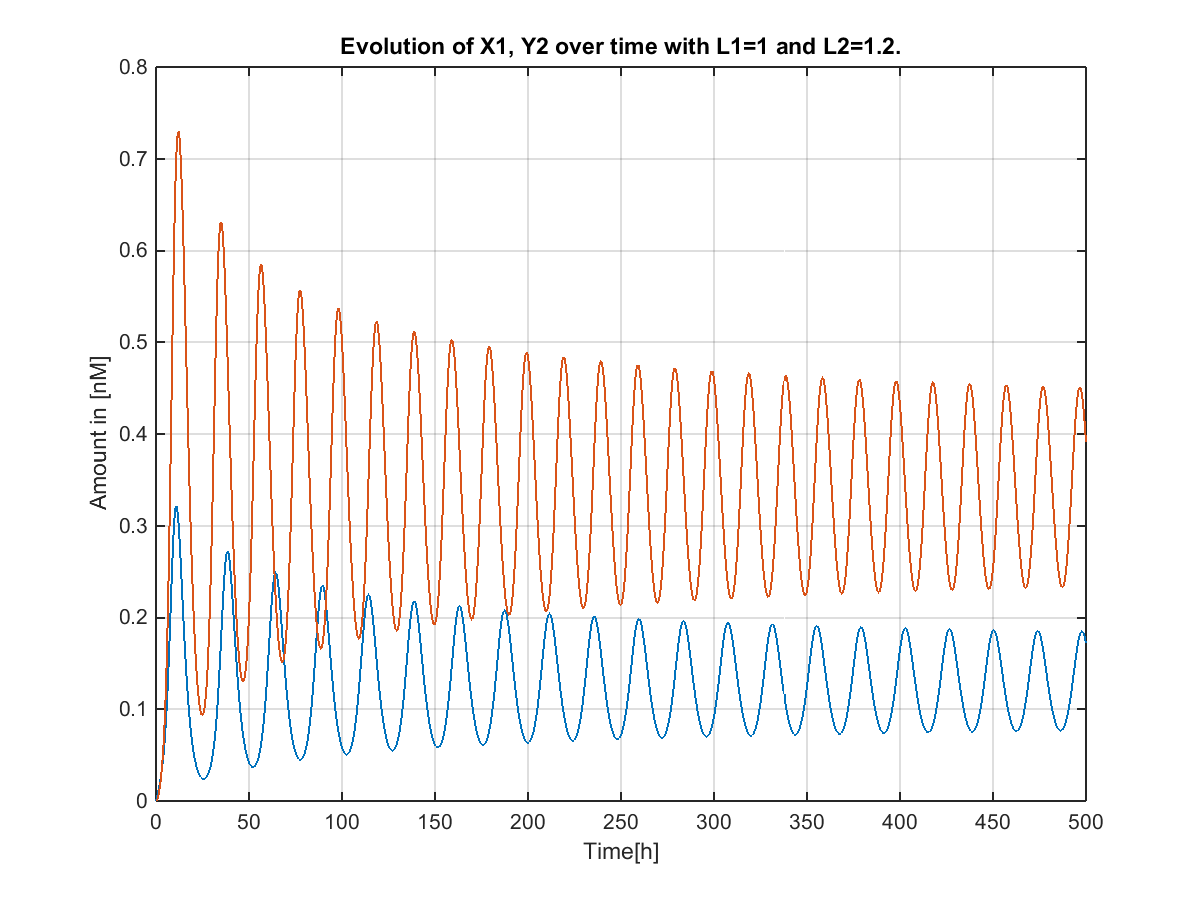
\includegraphics[width=\textwidth]{"../Miniprojet 2.0/Part B/B_2_graphs/B42.png}
	    \caption{$\lambda_1$ = 1, $\lambda_2$ = 1.2 [$h^{-1}$]}
	\end{subfigure}
	~ 
	\begin{subfigure}[b]{0.32\textwidth}
	    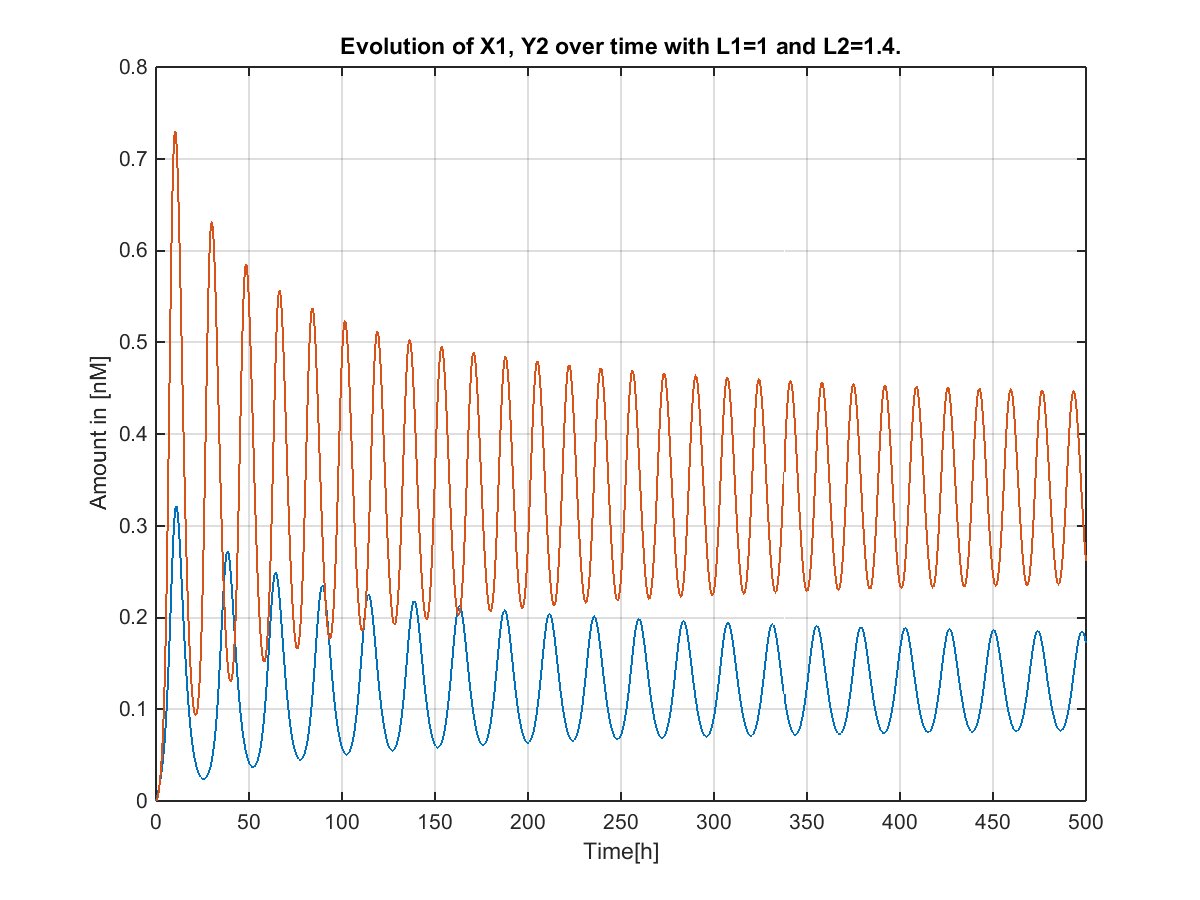
\includegraphics[width=\textwidth]{"../Miniprojet 2.0/Part B/B_2_graphs/B43.png}
	    \caption{$\lambda_1$ = 1, $\lambda_2$ = 1.4 [$h^{-1}$]}
	\end{subfigure}
	 
	\begin{subfigure}[b]{0.32\textwidth}
	    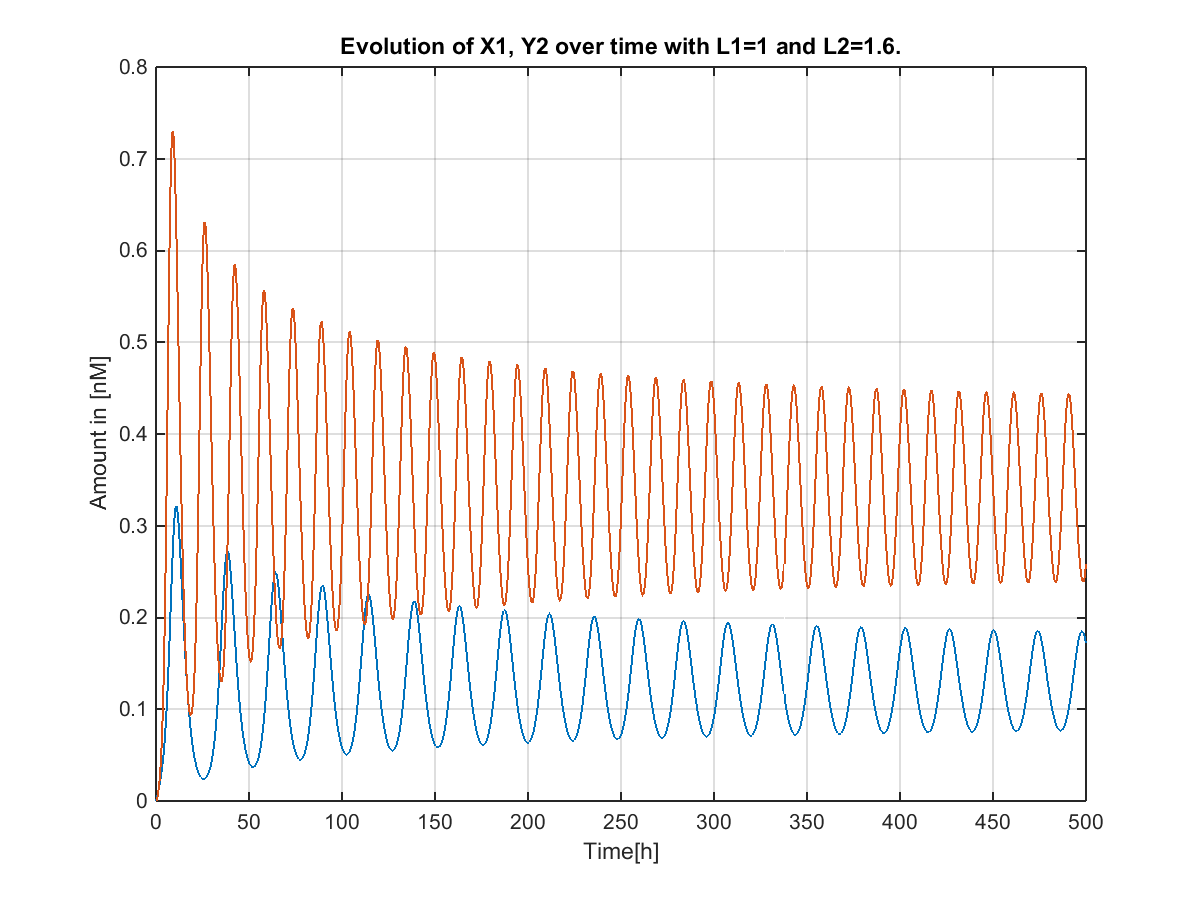
\includegraphics[width=\textwidth]{"../Miniprojet 2.0/Part B/B_2_graphs/B44.png}
	    \caption{$\lambda_1$ = 1, $\lambda_2$ = 1.6 [$h^{-1}$]}
	\end{subfigure}
	~ 
	\begin{subfigure}[b]{0.32\textwidth}
	    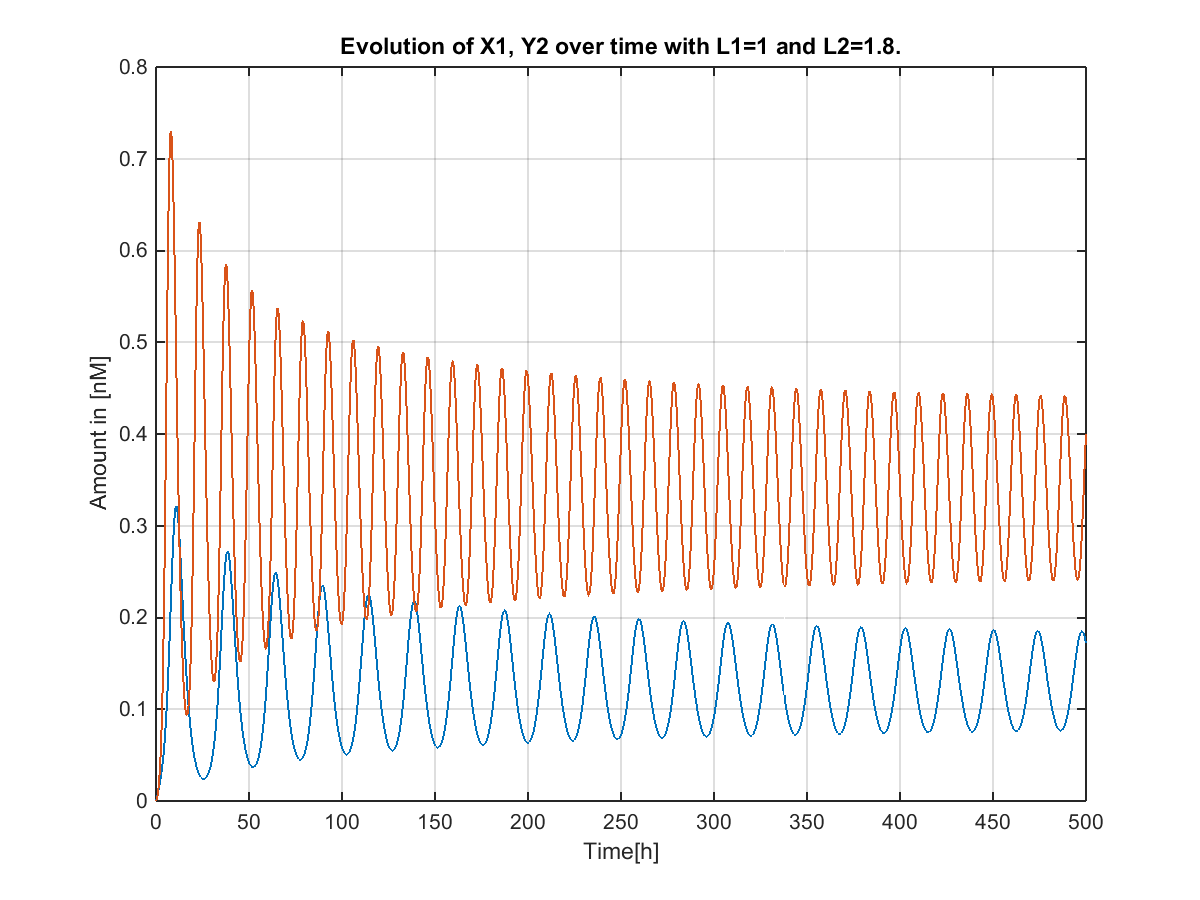
\includegraphics[width=\textwidth]{"../Miniprojet 2.0/Part B/B_2_graphs/B45.png}
	    \caption{$\lambda_1$ = 1, $\lambda_2$ = 1.8 [$h^{-1}$]}
	\end{subfigure}
	~ 
	\begin{subfigure}[b]{0.32\textwidth}
	    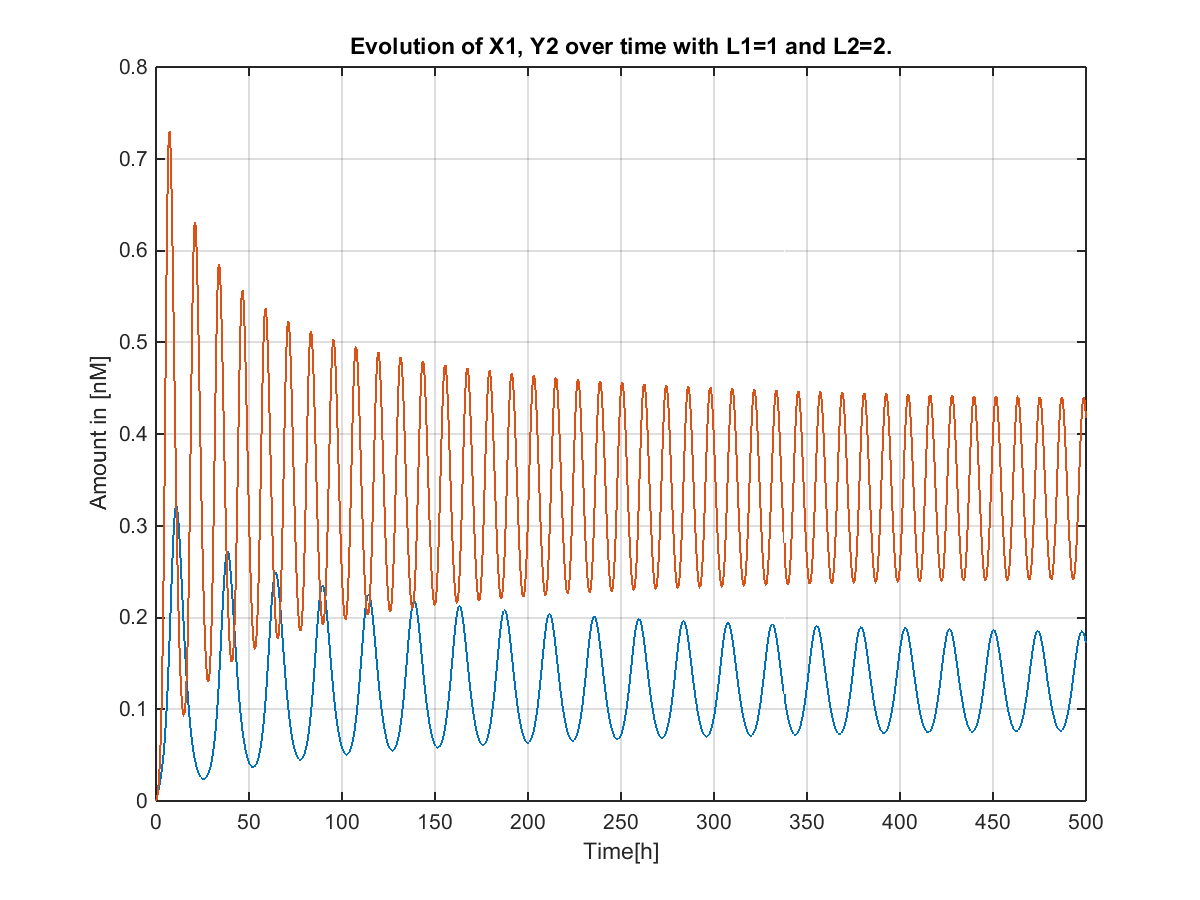
\includegraphics[width=\textwidth]{"../Miniprojet 2.0/Part B/B_2_graphs/B46.png}
	    \caption{$\lambda_1$ = 1, $\lambda_2$ = 2 [$h^{-1}$]}
	\end{subfigure}

	\caption{\orange{$X_1(t)$} and \blue{$Y_2(t)$} trajectories in a two-cells Model with $K=0$ (no synchronisation). The key observation to make here is that the signal of Y(t) is always slightly delayed to X(t).\\
	}
    \end{figure*}

    \begin{figure*}
    \centering
	\begin{subfigure}[b]{0.32\textwidth}
	    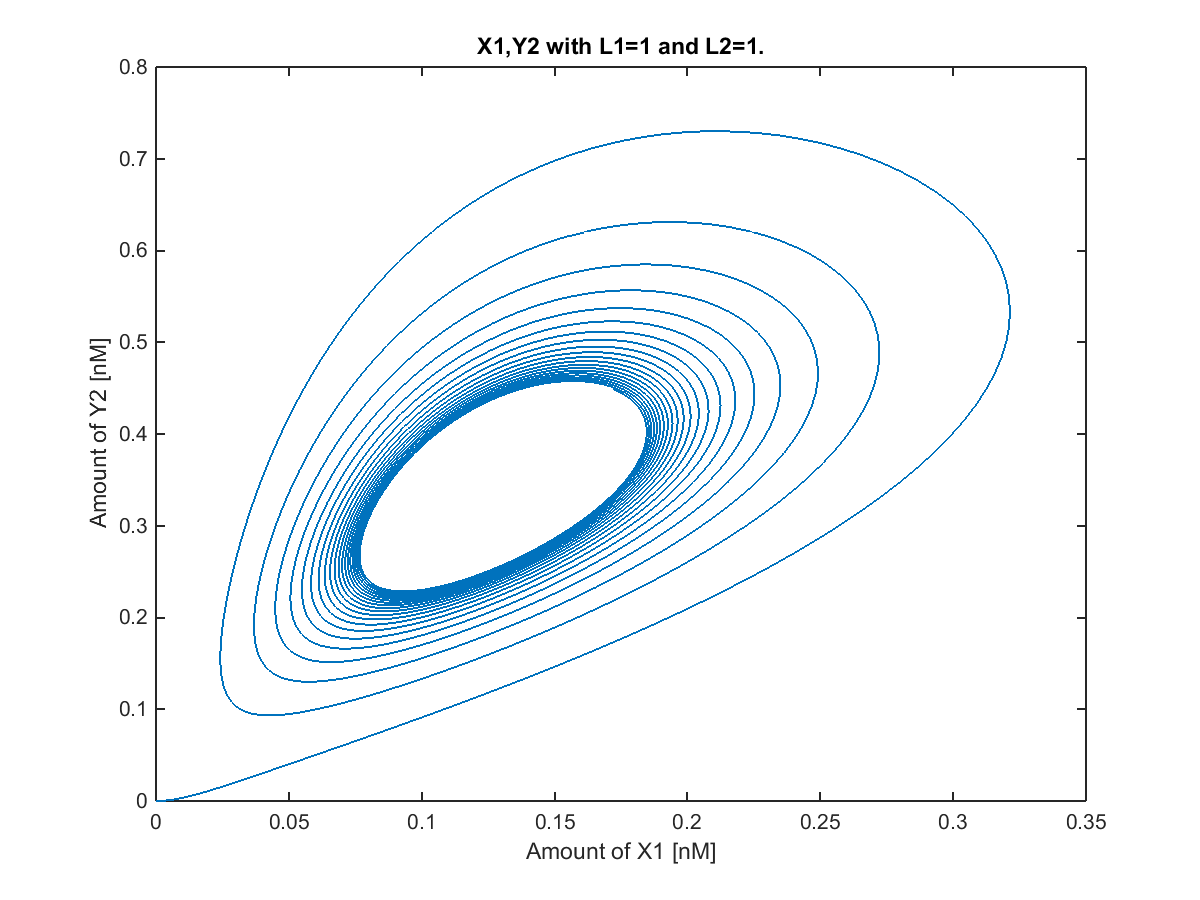
\includegraphics[width=\textwidth]{"../Miniprojet 2.0/Part B/B_2_graphs/B31.png}
	    \caption{$\lambda_1$ = 1, $\lambda_2$ = 1 [$h^{-1}$]}
	\end{subfigure}
	~ 
	\begin{subfigure}[b]{0.32\textwidth}
	    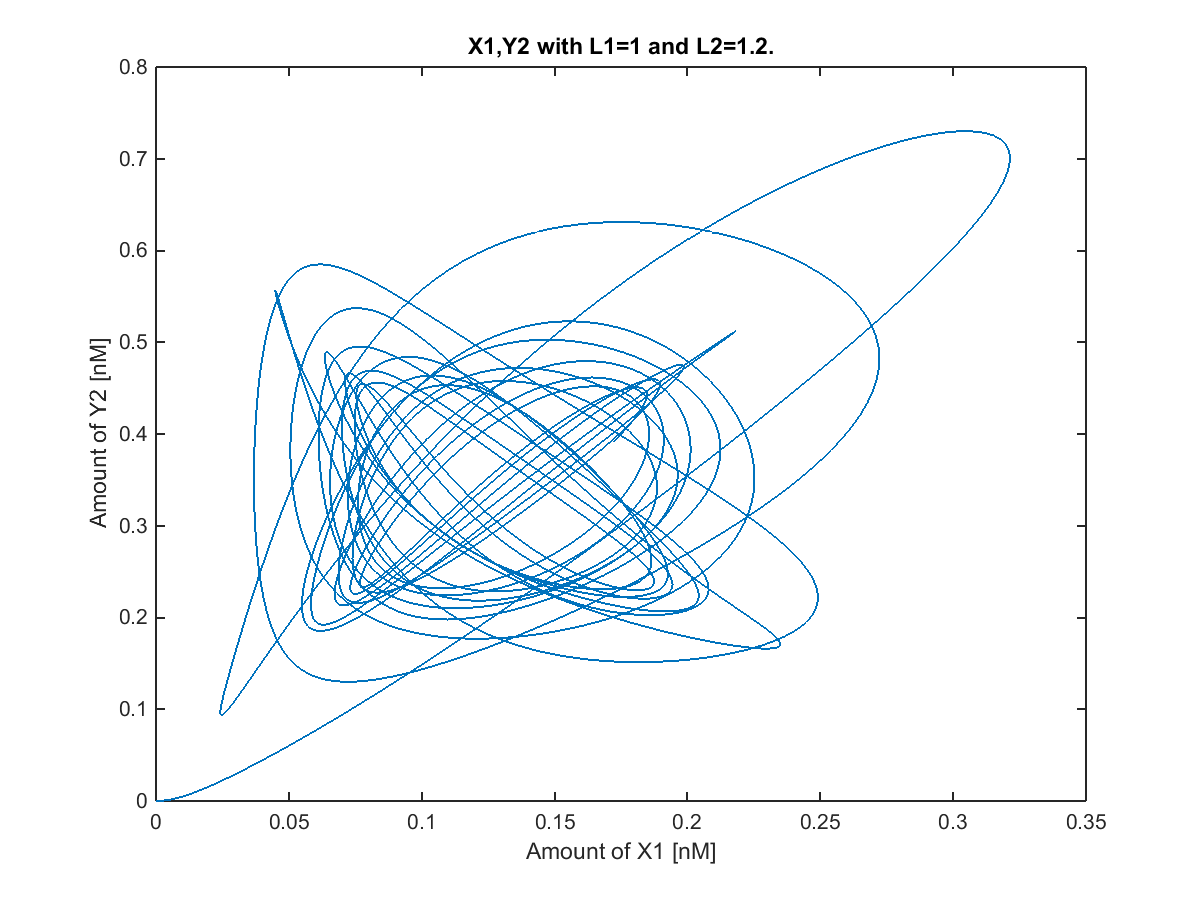
\includegraphics[width=\textwidth]{"../Miniprojet 2.0/Part B/B_2_graphs/B32.png}
	    \caption{$\lambda_1$ = 1, $\lambda_2$ = 1.2 [$h^{-1}$]}
	\end{subfigure}
	~ 
	\begin{subfigure}[b]{0.32\textwidth}
	    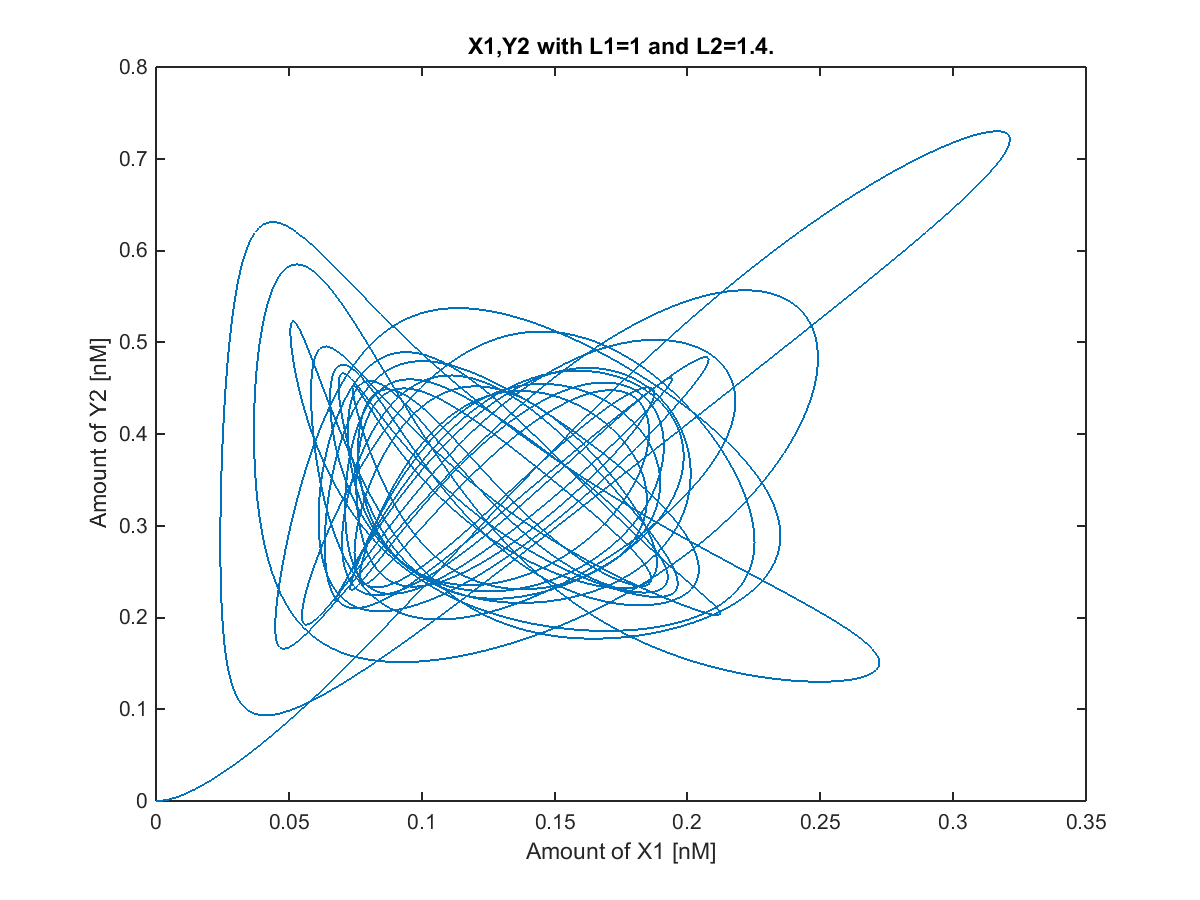
\includegraphics[width=\textwidth]{"../Miniprojet 2.0/Part B/B_2_graphs/B33.png}
	    \caption{$\lambda_1$ = 1, $\lambda_2$ = 1.4 [$h^{-1}$]}
	\end{subfigure}
	 
	\begin{subfigure}[b]{0.32\textwidth}
	    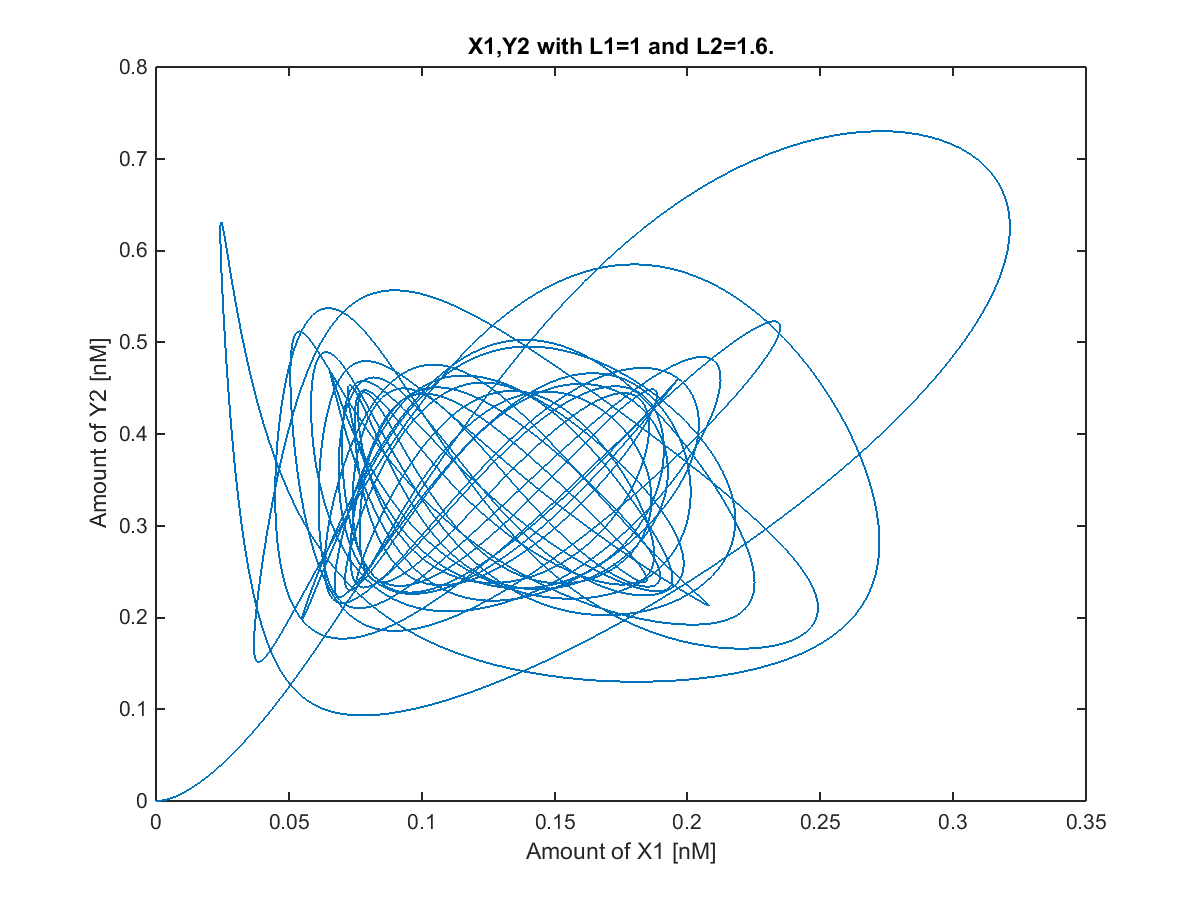
\includegraphics[width=\textwidth]{"../Miniprojet 2.0/Part B/B_2_graphs/B34.png}
	    \caption{$\lambda_1$ = 1, $\lambda_2$ = 1.6 [$h^{-1}$]}
	\end{subfigure}
	~ 
	\begin{subfigure}[b]{0.32\textwidth}
	    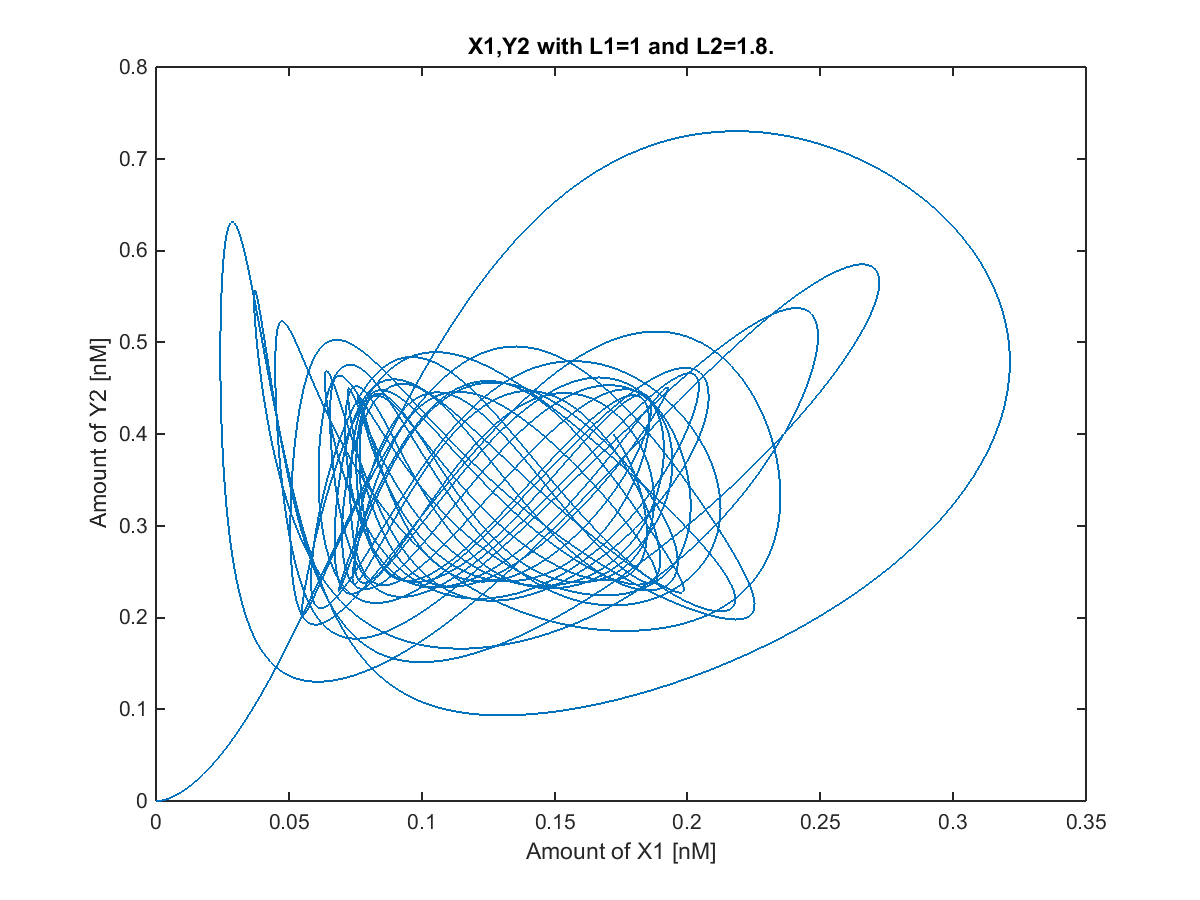
\includegraphics[width=\textwidth]{"../Miniprojet 2.0/Part B/B_2_graphs/B35.png}
	    \caption{$\lambda_1$ = 1, $\lambda_2$ = 1.8 [$h^{-1}$]}
	\end{subfigure}
	~ 
	\begin{subfigure}[b]{0.32\textwidth}
	    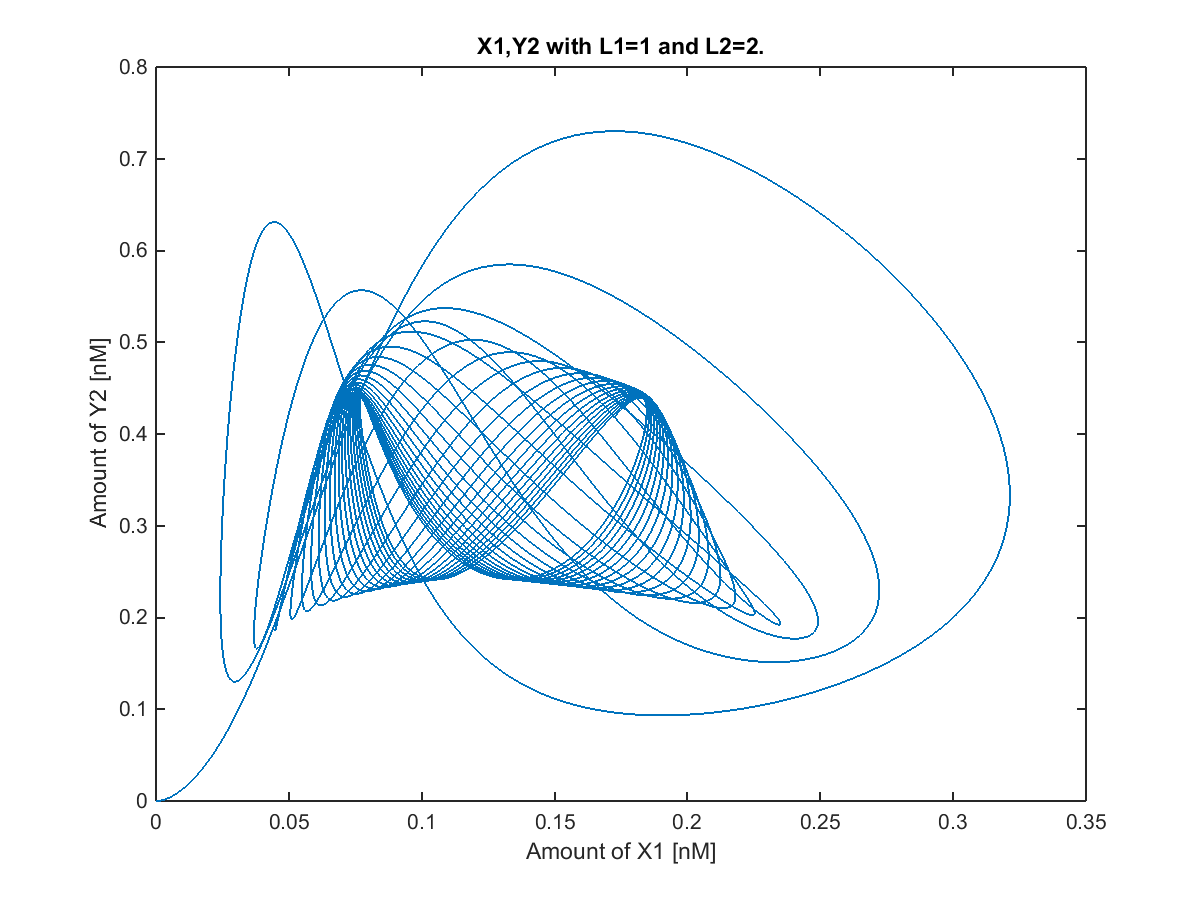
\includegraphics[width=\textwidth]{"../Miniprojet 2.0/Part B/B_2_graphs/B36.png}
	    \caption{$\lambda_1$ = 1, $\lambda_2$ = 2 [$h^{-1}$]}
	\end{subfigure}

	\caption{$X_1$ and $Y_2$ trajectories with varying $\lambda_i$ in a two-cells Model with $K=0$\\
	Once again, both cells tend to reach their limit cycles without any kind of interaction. The same observations as in Figure \ref{fig:11} can be made, except for the key difference in figure (a), where the fact that the two cells share the same period but are partially out of phase creates a limit cycle instead of a linear interaction.
	}
    \end{figure*}

    \begin{figure*}
    \centering
	    \begin{subfigure}[b]{0.35\textwidth}
	    \begin{equation*}R = \frac{\langle F^2 \rangle - {\langle F \rangle}^2}{\frac{1}{N}\sum_{i=1}^{N}(\langle V_i^2 \rangle - {\langle V_i \rangle}^2)} \end{equation*}
	    \hfill \\
	    \centering
	    \footnotesize{The Coefficient of Synchronization R is as the name suggests a measure of the synchronisation between $N$ different cells. This ratio can take any value between 0 and 1 as the variance of $F$ cannot exceed the mean value of the individual variances of $V_i$. \\
	    $R=1$ means very high synchronisation whereas $R=0$ means no synchronisation at all.}
	    \captionsetup{labelformat=empty}
	    \caption{\hfill \\ \hfill \\ \hfill \\} 	%ok this is freaking lame
	\end{subfigure}
	~
	\begin{subfigure}[b]{0.4\textwidth}
	    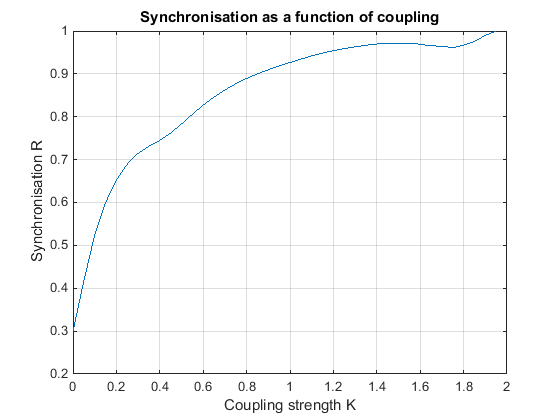
\includegraphics[width=\textwidth]{"../Miniprojet 2.0/Part B/B_N_3_graph_2.png}
	    \caption{\footnotesize{Value of $R$ depending on the Coupling Constant K}}
	\end{subfigure}
	\caption{We introduce the Coefficient of Synchronization R \\
	The plot shows some irregularity, but shows a clear trend. The higher the strength of the signal of V is (denoted by the factor K), the more the cells begin to oscillate in synchronisation.}
    \end{figure*}

    \begin{figure*}
    \centering
	\begin{subfigure}[b]{0.3\textwidth}
	    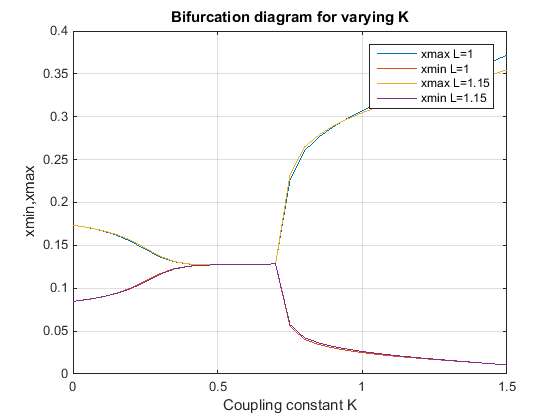
\includegraphics[width=\textwidth]{"../Miniprojet 2.0/Part B/B_3_bifurcation.png}
	    \caption{$\lambda_1=1$ $\lambda_2=1.15$ \\
	    and initial conditions $X_{i,0}=0~Y_{i,0}=0~Z_{i,0}=3~V_0={i,0}$}
	\end{subfigure}
	~
	\begin{subfigure}[b]{0.3\textwidth}
	    \includegraphics[width=\textwidth]{"../Miniprojet 2.0/Part B/B_3_bifurcation_2.png}
	    \caption{$\lambda_1=1$ $\lambda_2=1.5$ \\
	    and initial conditions $X_{i,0}=0~Y_{i,0}=0~Z_{i,0}=3~V_0={i,0}$}
	\end{subfigure}
	~ 
	\begin{subfigure}[b]{0.3\textwidth}
	    \includegraphics[width=\textwidth]{"../Miniprojet 2.0/Part B/B_2_marginally_less_stupid.png}
	    \caption{$\lambda_1=1$ $\lambda_2=1.15$ \\
	    and initial conditions $X_{i,0}=0~Y_{i,0}=0~Z_{i,0}=0~V_{i,0}=0$}
	\end{subfigure}

	\caption{Bifurcation diagram in a two-cells Model $X_{min}$ and $X_{max}$ plotted at time intervals $[9/10; 1]$ of $h_{max}=2000$h. We observe that if $K>$ a threshold value and if the difference in the periods of the two cells is high enough, the circadian behaviour of both cells dies. The reason for this is that the positive feedback loop has high sensitivity and tends to overload concentrations of $Z_i$ which in turn inhibit any production of $X_i$. This behaviour is further noticeable when the initial conditions are far from those of their limit cycles, as the cells enter tighter limit cycles ($\Delta X_{(c)} < \Delta X_{(a)}$)}
	\end{figure*}


    \begin{figure*}
    \centering
	\begin{subfigure}[b]{0.45\textwidth}
	    \includegraphics[width=\textwidth]{"../Miniprojet 2.0/Part B/100cells/100cells0_0.png}
	    \caption{$K=0.0$}
	\end{subfigure}
	~ 
	\begin{subfigure}[b]{0.45\textwidth}
	    \includegraphics[width=\textwidth]{"../Miniprojet 2.0/Part B/100cells/100cells0_5.png}
	    \caption{$K=0.5$}
	\end{subfigure}
	~ 
	\begin{subfigure}[b]{0.45\textwidth}
	    \includegraphics[width=\textwidth]{"../Miniprojet 2.0/Part B/100cells/100cells1_0.png}
	    \caption{$K=1.0$}
	\end{subfigure}
	 
	\begin{subfigure}[b]{0.45\textwidth}
	    \includegraphics[width=\textwidth]{"../Miniprojet 2.0/Part B/100cells/100cells1_5a.png}
	    \caption{$K=1.5$}
	\end{subfigure}
	~ 
	\begin{subfigure}[b]{0.45\textwidth}
	    \includegraphics[width=\textwidth]{"../Miniprojet 2.0/Part B/100cells/100cells1_5b.png}
	    \caption{$K=1.5$}
	\end{subfigure}

	\caption{$X_i(t)$ trajectories in a 100-Cells Model with initial conditions $X_{i,0}=0~Y_{i,0}=0~Z_{i,0}=3~V_{i,0}=0$ and $\lambda_i \sim N(0, 0.05)$. As excepted, with no coupling the cells are unable to synchronize leading to the loss of the signal in (a). Furthermore, with increasing $K$ the population synchronizes in 2-5 periods and in a decreasing period length pattern \red{u know talk english?}.}
    \end{figure*}


    \begin{figure*}[!htb] 		%oh my god this is so ugly pls don't look at me
	\captionsetup{labelformat=empty}
	\caption{\Huge{\textbf{Part C - Circadian Behaviour in the Brain}}}
    \end{figure*}

    \begin{figure*}
    \centering
	\begin{subfigure}[b]{\textwidth}
	    \includegraphics[width=\textwidth]{"../Miniprojet 2.0/Part C/C_2_figure_1.png}
	    \caption{$K=0.0$}
	\end{subfigure}
	 
	\begin{subfigure}[b]{\textwidth}
	    \includegraphics[width=\textwidth]{"../Miniprojet 2.0/Part C/C_2_figure_2.png}
	    \caption{$K=0.3$}
	\end{subfigure}
	\caption{raraara}
    \end{figure*}

\end{document}
